% !TEX root = thesis.tex
{
\cleardoublepage% Move to first page of new chapter
\let\cleardoublepage\relax% Don't allow page break
\noindent \small{Based on: \emph{Probabilistic modelling of general noisy multi-manifold data sets}, Canducci~M., Ti\v{n}o~P., Mastropietro~M. \citet{Canducci2021}.
Part of this work has been carried out during the planned SUNDIAL secondment at the Computer Science Department of the University of Birmingham.
}
\chapter{Low-dimensional manifolds}
\label{ch:manifolds}
}

\abstract{
The intrinsic nature of noisy and complex data sets is often concealed in low-dimensional structures embedded in a higher dimensional space.
%Number of methodologies have been developed to extract and represent such structures in the form of manifolds (i.e. geometric structures that locally resemble continuously deformable intervals of $\mathbb{R}^j$ \footnote{$j$ is the manifold dimensionality.
%Mathematically, continuous deformation corresponds to homehomorphism: one-to-one continuous mapping with continuous inverse.}).
% Usually a-priori knowledge of the manifold's intrinsic dimensionality is required.
% Additionally, their performance can often be hampered by the presence of a significant high-dimensional noise aligned along the low-dimensional core manifold.
In real-world applications, the data can contain several low-dimensional structures of different dimensionalities.
We propose a framework for dimensionality estimation and reconstruction of multiple noisy manifolds embedded in a noisy environment.
%To the best of our knowledge, this work represents the first attempt at detection and modelling
%of a set of coexisting general noisy manifolds by uniting two aspects of multi-manifold learning:
%the recovery and approximation of core noiseless manifolds and the construction of their probabilistic models.
%The easy-to-understand hyper-parameters can be manipulated to obtain an emerging picture of the multi-manifold structure of the data.
% We demonstrate the workings of the framework on two synthetic data sets, presenting challenging features for state-of-the-art techniques in Multi-Manifold learning.
% The first data set consists of multiple sampled noisy manifolds of different intrinsic dimensionalities, such as M\"{o}bius strip, toroid and spiral arm. The second one is a topologically complex set of three interlocked toroids.
% Given the absence of such unified methodologies in the literature, the comparison with existing techniques is organized along the two separate aspects of our approach mentioned above, namely manifold approximation and probabilistic modelling.
The framework is then applied to a complex data set containing simulated gas volume particles from a particle simulation of a dwarf galaxy interacting with its host galaxy cluster.
Detailed analysis of the recovered \mbox{1-D} and 2-D manifolds can help us to understand the distribution of various physical quantities in such complex systems.
The technique allows to isolate the evolution of quantities around tails of a simulated jellyfish galaxy, so that of star formation regions and the mixing of galaxy gas and cluster gas can be studied.
}
\section{Introduction}


Dimensionality reduction and Density Estimation of raw data, are commonly used tools to extract information from complex and noisy data sets.
Due to dependencies among measured attributes of real world data,
the data is often distributed along low-dimensional structures in a higher dimensional measurement space.
This realisation has driven the development of a variety of Manifold Learning algorithms.
Principal Component Analysis \citep[PCA, ][]{Pearson1901} is a well understood and widely used linear dimensionality reduction scheme.
%\Marco{It can be considered the progenitor of Manifold Learning, where the data is assumed to lie on a multivariate Gaussian and the recovered principal components capture the variance of the data along orthogonal directions.}
However, by design, PCA cannot appropriately capture non-linear low-dimensional structures.
% This lack of flexibility has been addressed by non-linear dimensionality reduction algorithms such as Isomap \cite{Tenenbaum2319}
% and Locally Linear Embedding \citep[LLE][]{Roweis00nonlineardimensionality},
% where the manifold is approximated by a neighbourhood graph and a neighbouring preserving map respectively.
% Both methods take advantage of the definition of a manifold as a locally linear low dimensional structure of dimension $j$.

% Many other Manifold Learning algorithms aiming to provide suitable approximations to low-dimensional data manifold have been proposed.
% Examples include Laplacian eigenmaps \citep{Belkin01laplacianeigenmaps},
% Hessian eigenmaps \citep{Donoho5591},
% Local Space Tangent Alignment \citep[LSTA, ][]{Zhang02principalmanifolds},
% C-Isomap \citep[an extension of Isomap to conformal embeddings][]{Silva:2002:GVL:2968618.2968708},
% NMDS \citep[non-metric formulation of Multidimensional Scaling (MDS)][]{doi:10.1002/bs.3830040308, Cox2008, Kruskal1964},
% Riemannian Manifold Learning \citep[RML, ][]{10.1109/TPAMI.2007.70735}.

% In \cite{boissonnat:hal-01615863} (and bibliographic references therein) a different angle, based on computational geometry,
% has been proposed in order to extract low-dimensional manifolds from data samples.
% Here, simplicial complexes (such as Delaunay triangulations, $\alpha$-complexes and filtrations)
% are used for manifold reconstruction.
% With these techniques it is possible to infer geometrical and topological properties of data points
% that uniformly sample a single manifold embedded in a higher dimensional space.

% While such techniques are potentially powerful and theoretically well grounded,
% their capability to naturally handle high-dimensional noise aligned along low-dimensional manifolds is limited.
% Besides the sensitivity to the noise issues, it is often required that the intrinsic data dimensionality is known a priori.

Generative Topographic Mapping \cite[GTM, ][]{Bishop1998GTMTG} was proposed as a probabilistic formulation of the Self-Organizing Map \citep{Kohonen1982}.
Its main advantage is that instead of treating noisy manifold as a core low-dimensional manifold to be discovered,
plus some ``noise" around it that somehow needs to be dealt with,
it formulates a consistent manifold-aligned density model in the form of a constrained mixture of Gaussians.
The location parameters (means) of the Gaussian components are constrained to lie on a smooth manifold
-- most commonly a smooth image in the data space of a two-dimensional interval (latent space).
%The original GTM formulation is trained in the maximum likelihood framework using the the Expectation-Maximization (E-M) algorithm \citep{10.2307/2984875}.
%Because of the sensitivity to initialization, a suitable initialization is required (e.g, using PCA).
% Bayesian formulations of GTM have also been proposed \cite{Olier2008VariationalBG}.

%Other global density estimators, whether non-parametric, e.g. Parzen windows \cite{parzen1962estimation}
%(and its extensions such as Manifold Parzen Windows \cite{NIPS2002_2203}, Fast-Parzen Windows \cite{5178637}),
%or semi-parametric, e.g. Infinite Gaussian Mixture model\cite{10.5555/3009657.3009736},
%are not designed to extract a representation of the embedded low-dimensional structures.
%They also may be computationally expensive to train and/or evaluate.

% To deal with complex data sets, where several manifolds of different dimensionalities can co-exist,
% generalizations of the previous methods have been developed:
% Multi-Manifold Discriminant Analysis (MMDA, \cite{Yang:2011:MDA:1963661.1963809}),
% Sparse-Manifold Clustering and Embedding (SMCE,\cite{NIPS2011_4246}),
% Multi-Manifold Isomap (M-ISOMAP\cite{Fan2012IsometricML}),
% Multi-manifold Proximity Embedding  (MPE,\cite{Fan:2016:EIM:2903049.2903101}),
% Multi-Manifold LLE (MM-LLE,\cite{Hettiarachchi:2015:MLL:2791619.2792198}),
% S-Isomap++ \cite{2017arXiv171006462M},
% Hierarchical GTM \cite{Tino_PAMI_2002}.
% However, based on the same assumptions as their predecessors, the methods still need to be informed
% about the dimensionalities of the different manifolds
% and struggle when dealing with topologically complex, noisy structures}.

In \citet{Canducci2021} we propose a framework for automated dimensionality estimation and reconstruction
of multiple noisy manifolds embedded in a noisy environment called \emph{Abstract Generative Topographic Mapping} (AGTM).
%\begin{itemize}
%  \item it proposes a new robust dimensionality index estimation for data points,
%  \item through a dedicated manifold crawling mechanism it allows for completely abstract manifold representations in the GTM latent space (instead of a regular grid), and
%  \item it has Gaussian noise components naturally aligned along the manifold, unlike the spherical noise models in the original GTM and \cite{10.1007/978-3-540-87481-2_37}.
%\end{itemize}
%Manifold aligned noise models in GTM were also considered in \cite{Bishop1998DevelopmentsOT},
%but under the assumption of simple latent space structure in the form of $j$-dimensional interval.
%The key idea was to impose larger and smaller variances in directions locally parallel and perpendicular, respectively, to the manifold.
Since our latent space is a discrete structure (abstract graph representing a skeleton of a given manifold),
we formulate local noise models through kernel based estimates of the local covariance matrix of the data,
with trainable scale parameter to allow for optimized overlapping of the neighbouring Gaussian components.
The work is inspired by \cite{10.1007/978-3-540-87481-2_37}, but extends and generalizes it, so that densities aligned along arbitrary manifolds (even non-orientable ones such as M\"{o}bius strip) can be captured,

The detailed aspects of AGTM will not be described in this thesis, because its treatment is not suitable for this context.
However, after the identification of the low-dimensional manifold as in \citet{Canducci2021}, instead of the probabilistic one, we'll use the SPH approach to estimate densities to compute physical quantities along the manifolds.

This work is the product of the collaboration in the SUNDIAL network between the Birmingham and the Gent node.
It should be clear that the original mathematical treatment of dimensionality estimation and AGTM have been authored by the Birmingham node.
My direct contributions to the work are the idea of analysis of jellyfish tails, the development of  independent code to test the manifold analysis,
the scientific questions driving the application of the method, supervision on the implementation, the proposal of physical quantities to be analyzed from the simulation and their physical interpretation.

%This is achieved by replacing the simple Euclidean latent space (generally parametrized as a discretized interval of $\mathbb{R}^j$)
%with an abstract graph reflecting the topology of the data manifold that, when embedded in the data space,
%provides a manifold skeleton around which the noise models can be organized.

%Our work presents a radical reformulation of GTM to capture and model low-dimensional general noisy manifolds
%through a dedicated abstract graph-structured latent space reflecting the core manifold structure, specific to each noisy manifold.
% \citet{Bacciu13} present another radical generalization of GTM in the reverse direction -
% this time keeping the original simple latent space structure, but allowing for abstract structure in the data space - the space of trees.

%The paper has the following organization: in section \ref{sec:Methodology} we set up the scene,
%explain the broad outline of the methodology and introduce the synthetic data set on which different steps of the methodology will be demonstrated.
%Section \ref{sec:AGTM} introduces the core model of our methodology, Abstract~GTM (AGTM),
%representing density aligned along a single manifold.
%We explain how the abstract latent space graph representing topology of the data manifold is
%extracted through manifold crawling and how this graph is then embedded in the data space along with the suitable set of noise models.
%We also show how to calculate local curvature at the edges of the embedded graph,
%taking advantage of the smooth manifold description provided by AGTM.
%Section \ref{sec:D_Index} defines our notion of dimensionality index for individual points.
%We also offer a computationally efficient alternative to Multi-Manifold Crawling.
%The price to pay for gains in efficiency is weaker detection stability of low dimensional manifold entities buried in the data.
% Section \ref{sec:Comparison} presents an experimental comparison on two synthetic data sets of our methodology
% with alternative multi-manifold learning and probabilistic modelling methods.
%Even though our methodology aims to provide density models of multiple low-dimensional manifolds buried in the data,
%we organise the comparative experiments separately for the multi-manifold capture and probabilistic modelling aspects of our work.
%This is because to the best of our knowledge, no other method exists that can simultaneously recover low dimensional
%representations of an unknown number of manifolds while building their probabilistic models.

%Our main contributions can be summarized as follows:
%\begin{itemize}
%    \item Formulation of a new dimensionality index assigned to individual points based on which point cloud can be partitioned into background points and sets representing cloud points organised along noisy low-dimensional manifold structures;
%    \item Development of a recursive crawling algorithm for the extraction of multiple low-dimensional, noisy manifolds embedded in a higher dimensional space: Multi-Manifold crawling;
%    \item Extension of GTM's applicability to a broad class of manifolds (\eg{} non-orientable or closed manifolds) by reformulating the latent space as an abstract graph and introducing a manifold-aligned noise attached to the embedded nodes of the latent graph: Abstract GTM.
%    The abstract latent space and its embedding allows us to {\em understand the important global structural features of the underlying manifolds}
%%     - an important aspect of our methodology bringing manifold learning under the umbrella of Artificial Intelligence.
%\end{itemize}

The methodology is applied in section \ref{sec:Ex_JellyFish} to a numerical simulation of a dwarf galaxy falling into the gaseous halo of a Fornax-like cluster, a snapshot of the simulation ID 69 described in Chapter~\ref{ch:simulations}.
{The point cloud generated by the simulation presents non linear, noisy, low dimensional structures,
providing for an ideal test bed for our methodology.}
We extract and model two of the most significant manifolds, suggesting a possible scenario for formation of new stars in such a disrupted dwarf galaxy.
% TODO mention the quantities varying along the manifold.

\section{Methodology} \label{sec:Methodology}
We refer to \citet{Canducci2021} for the thorough mathematical presentation of the technique.
Here we sketch the main ideas and we set up the scene in order for the reader to understand the overall methods used.
In the following we give a brief outline of our methodology to robustly detect the manifolds.

\subsection{Diffusion filtering} \label{sec:SAF}
Consider a point cloud
\[\mathcal{Q} =\{\vect{t}_1, \vect{t}_2,...,\vect{t}_L\},\quad \vect{t}_i \in \mathbb{R}^d\]
containing points sampled from an unknown number of noisy lower-dimensional manifolds embedded in a noisy environment (\eg{} points generated from a broad $d$-dimensional distribution).
We first apply a physics-based diffusion method, Structure-Aware Filtering Technique \citep[SAF,][]{Wu2018}, that collapses points in close vicinity of dense structures onto them, resulting in a diffused data set:
\[\tilde{\mathcal{Q}} =\{\tilde{\vect{t}}_1, \tilde{\vect{t}}_2,...,\tilde{\vect{t}}_L\},\quad \tilde{\vect{t}}_i \in \mathbb{R}^d.\]
% NOTE how SAF works?
% It defines a velocity as the gradient of the smoothed density (you can use two kernel, one for repusion, one for attraction) and advects points until convergence.
The SAF method moves points towards high density regions, enabling points in the vicinity of a noisy manifold to migrate towards its ``spine" or ``mean surface".

Assuming that the data structures to be modeled are more densely sampled than the noisy environment
we first filter the data sets $\mathcal{Q}$ and $\tilde{\mathcal{Q}}$ by removing point couples $(\vect{t}_i,\tilde{\vect{t}}_i)$ that have sparse neighbourhood in \emph{both} $\mathcal{Q}$ \emph{and} $\tilde{\mathcal{Q}}$.
In particular, around each $\vect{t}_i$ and $\tilde{\vect{t}}_i$ we construct a hyperball $\mathcal{B}(\vect{t}_i;r)$ and $\mathcal{B}(\tilde{\vect{t}}_i;r)$ in $\mathbb{R}^d$ of radius $r>0$.
In case a point $\vect{t}_i$ lies further apart from a manifold, both hyperballs will be sparsely populated.
Hence, if both $\mathcal{B}(\vect{t}_i;r)$ and $\mathcal{B}(\tilde{\vect{t}}_i;r)$ contain less points than a pre-specified threshold $\tau>0$ the points $\vect{t}_i$ and $\tilde{\vect{t}}_i$ are removed from their corresponding data sets.

%\subsection{Manifold analysis overview}
Following this, the first task in capturing the multi-manifold structure in $\tilde{\mathcal{Q}}$ is to estimate local dimensionality of the cloud point around each $\tilde{\vect{t}}_i$
in the form of a \emph{dimensionality index} $\delta_i$ (section \ref{sec:D_Index}).
Using the dimensionality indices, we partition the data into subsets $\tilde{\mathcal{Q}}_j$ according to the local dimensionalities $j=1,2,...,d$.

Since $\mathcal{Q}_j, \tilde{\mathcal{Q}}_j$ can contain several distinct sampled manifolds of dimensionality $j$,
we use a dedicated \emph{manifold crawling} procedure operating on $\tilde{\mathcal{Q}}$ to separate the individual manifolds (section \ref{sec:Crawling}).
Moreover, the crawling also produces for each manifold a graph structure embedded in $\mathbb{R}^d$ representing a piece-wise linear ``skeleton" approximation of the spine of the noisy manifold.
%To isolate a low dimensional manifold and generate the topography of the latent space containing all the information about a detected manifold the \emph{manifold crawling} algorithm has been developed \citep[see section 3.2 of][]{Canducci2021}.


%For every manifold, the associated graph will then function as an abstract latent space of a generalized form of Generative Topographic Mapping (GTM) \cite{Bishop1998GTMTG} that we call \emph{Abstract GTM} (AGTM).
%Using points in $\tilde{\mathcal{Q}}$, the generalized GTM produces manifold aligned density models. %(section \ref{subsec:GTM}).

%Finally, if a single summary model is required, density models of all detected manifolds (AGTMs) can be grouped together in a hierarchical mixture model \cite{Tino_PAMI_2002} representing in a concise manner the global density of the low-dimesional structures in the dataset $\tilde{\mathcal{Q}}$.

\subsection{Dimensionality estimation} \label{sec:D_Index}
Around each $\tilde{\vect{t}}_i \in \tilde{ \mathcal{Q}}$ we perform local Principal Component Analysis (PCA) using points from  $\mathcal{B}(\tilde{\vect{t}}_i;r) \cap \tilde {\mathcal{Q}}$, obtaining eigenspectrum
\[\lambda_{i,1} \ge \lambda_{i,2} \ge ... \ge \lambda_{i,d}.\]

%The dimensionality index of $\tilde{\vect{t}}_i \in \tilde{ \mathcal{Q}}$ used in \cite{10.1007/978-3-540-87481-2_37} (limited to 3-dimensional data) was obtained as
%\begin{equation}
%	\delta^O_i = \argmax_j S_{i,j}
%\end{equation}
%where $ S_{i,1} = {\lambda}_{i,1} - {\lambda}_{i,2}$, $S_{i,2} = 2 ({\lambda}_{i,2} - {\lambda}_{i,3})$ and $S_{i,3} = 3 {\lambda}_{i,3}$.

We suggest a general method for computing dimensionality index of points distributed in spaces of arbitrary finite dimension $d$, based on renormalized eigenvalues,
\[
\tilde{\lambda}_{i,j} = \frac{\lambda_{i,j}}{\sum_{k=1}^d \lambda_{i,k}},
\]
viewed as ``likelihoods" of different dimensionalities $j$ of the cloud of points around $\tilde{\vect{t}}_i$.
\paragraph{Simplex}
Note that
$\tilde{\Lambda}_i = (\tilde{\lambda}_{i,1}, \tilde{\lambda}_{i,2},\dots,\tilde{\lambda}_{i,d})$
lies in the ($d-1$)-dimensional simplex $\mathcal{S}_0$ with vertices:
\begin{align*}
\s_1 &= (1, 0, 0, \dots,0),\\
\s_2 &= (1/2, 1/2, 0, \dots, 0),\\
\s_3 &= (1/3, 1/3, 1/3, \dots, 0),\dots\\
\s_d &= (1/d, 1/d, 1/d, \dots ,1/d).
\end{align*}


%The simplex $\mathcal{S}_0$ is a subset of the standard simplex $\mathcal{S}$ with vertices equal to the standard basis
%\begin{align*}
%\e_1 &= (1, 0, 0, \dots, 0),\\
%\e_2 &= (0, 1, 0, \dots, 0),\\
%&\vdots\\
%\e_d &= (0, 0, 0, \dots, 1).
%\end{align*}
%Considering $\mathcal{S}$ as the simplex of multinomial distributions,
%the appropriate Riemannian geodesic distance is the Fisher distance % FIXME why the Fisher?
%\citep{Lebanon:2005:RGS:1087529}.
It is useful to see $\mathcal{S}_0$ as a subset of the the simplex of multinomial distributions, so that for any point of the simplex, $\tilde{\Lambda}_k \in \mathcal{S_0}$,
we will compute its distance from the vertex $\s_j$ using the Fisher distance \citep{Lebanon:2005:RGS:1087529}:
\begin{equation}
	\label{eq:FishDist}
	d_J(\tilde{\Lambda}_k,\s_j) = 2\arccos{\left(\sum_{i=1}^{d} \sqrt{(\tilde{\lambda}_{ki}\, s_{ji})}\right)}.
\end{equation}
We therefore assign to each point $\tilde{\vect{t}}_i$ of the dataset a
dimensionality index $\delta_i$ as the index of the closer (assuming the $d_J$ distance metric) vertex of the simplex:
%Note that the vertex $\s_j$ of $\mathcal{S}_0$ corresponds to the ideal normalized eigen-spectrum of a $j$-dimensional neighbourhood.
%Hence, we will quantify the degree to which the neighbourhood of $\tilde{\vect{t}}_i$ resembles a $j$-dimensional hyperplane in $\RR^d$ by the closeness of $\tilde{\Lambda}_i$ to $\s_j$
%in terms of the geodesic distance
%\eqref{eq:FishDist},
\begin{equation}\label{eq:idxHard}
	\delta_i = \argmin_j d_J(\tilde{\Lambda}_i,\vect{s}_j).
\end{equation}

In \citet{Canducci2021} also a ``soft" and spatially smoothed version of the dimensionality index is proposed.

\begin{figure}[ht!]
  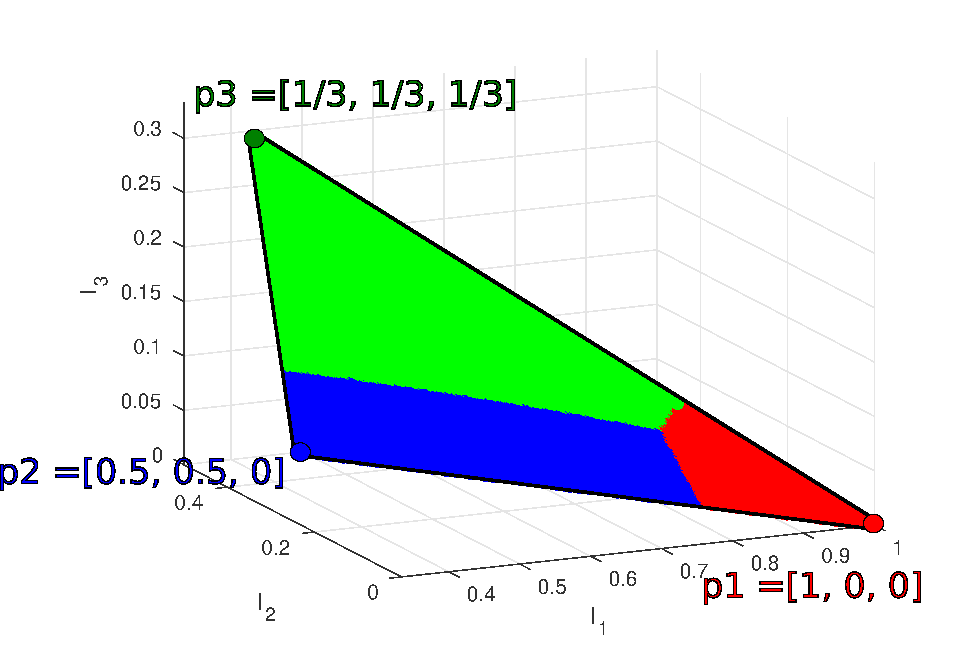
\includegraphics[width=\textwidth]{Figures_png/Classified_Simplex_lowRes.pdf}
  \caption{Simplex $\mathcal{S}_0$ in three dimensions. p1, p2 and p3 are the analogous of the $\s_1, \s_2, \s_3$ vertexes. The three parts of the simplex are coloured depending on the minimum distance vertex using the Fisher metric \eqref{eq:FishDist}.}
  \label{fig:simplex}
\end{figure}

\subsection{Crawling} \label{sec:Crawling}
%\begin{figure}[th!]
%\begin{subfigure}[t]{\textwidth}
% \includegraphics[width=\textwidth]{Figures_png/RanStrip_Whole.png}
% \caption{}
% \label{subfig:MGraph}
%\end{subfigure}
%\begin{subfigure}[t]{\textwidth}
% \includegraphics[width=\textwidth]{Figures_png/Mobius_Whole.png}
% \caption{}
% \label{fig:Mobius_Whole}
%\end{subfigure}
%%  \subfloat[][]{\label{subfig:MGraph}\includegraphics[width = 0.9\textwidth]{Figures_png/RanStrip_Whole}} \\
%%  \subfloat[][]{\label{subfig:MGraph_Emb}\includegraphics[width = 0.9\textwidth]{Figures_png/Mobius_Whole}}
%\caption{ (a) shows the classic GTM setup;
%the leftmost panel is a representation of the latent space discretized in a grid of points $x_i$.
%The $j$-dimensional interval $[-1,+1]^j$ is mapped through the parametrized function $\vect{y}(\mathcal{X};W)$ onto the data space with a spherical Gaussian centered on each point assumed as noise.
%The noise model aims at describing the true distribution of points in the data space (rightmost panel).\\
%(b) is a sketch of \emph{AGTM}.
%The latent space is substituted with an abstract graph, shown here for the M\"obius strip, together with its topological representation (the two arrows pointing in opposite directions on the shortest edges of the graph).
%Function $f(\cV;\W)$ maps the graph onto the data space and manifold-aligned noise models are estimated on each graph's node $\overline{\vect{v}}_i$ % FIXME why f is not bold?
%The true noisy distribution is displayed in the rightmost panel.}
%\end{figure}


We leave once again the mathematical details to \citet{Canducci2021} for a clear and thorough exposition, and we highlight here the fundamental ideas.
% TODO This crawling is part of a more general technique to extract probabilistic models of filaments/manifolds and smooth the extracted filament by training a maximum likelihood.
%TODO Difference with Disperse. We have instead a Knowledge aware starting point.

After having identified the subsets of points belonging to manifolds of different dimensionalities, for each dimension we would like to isolate the (possibly multiple) embedded manifolds they can contain.
The goal is to create a latent space containing all the information about a detected manifold $\cM$ embedded in a higher dimensional data space.
%If we then define a probability distribution $p(v)$ on the latent-variable space, this will induce a distribution
%$p(\vect{t}|\f)$ in the data space, which is what we are seeking in the end.
%The assumed distribution in the data space is a Gaussian with the local manifold-aligned covariance matrix $\Sigma$ computed as:
%\[...\]

The mapping $\f: \cV \to \RR^d$ from the latent space to the data space is, following \citet{Bishop1998GTMTG},
a nonlinear model, linear in parameters.
The latent space grid structure can be represented by an abstract undirected graph $\cG = (\cV,\cE)$, where each grid point corresponds to a vertex $v_i \in \cV$ and edges $e_{ij} \in \cE$ are connecting vertices corresponding to neighbouring grid points.
In particular, the image of a vertex $v \in \cV$ %under $\Phi = (\phi_1,..., \phi_M)^\top$
is obtained as $\overline{\vect{v}}_i = \f(v)$ operating on the latent space $\cG$ \citep[see section 3.1 of][for details]{Canducci2021}.
The goal of the crawling is to create a manifold skeleton formed by the embedded graph
$\overline{\cG} = (\overline{\cV},\overline{\cE})$.%, where the vertexes
%$\overline{\cV} = \{ \bar{\vect{v}}_i, ..., \bar{\vect{v}}_K\}$ and the edges
%$\overline{e}_{ij} \in \overline{\cE}$. % whenever ${e}_{ij} \in {\cE}$.
%\begin{equation}
%  \overline{\vect{v}}_i = \f(v;\W) = \W \vect{\Phi}(v),
%  \label{eq_f}
%\end{equation}
%where $\mathbf{W}$ is a $d \times M$ matrix of weights and $\vect{\Phi}$ is a set of basis functions $\phi_m: \cV \to \RR$, $m=1,2,...,M$,

\paragraph{Manifold crawling}
Briefly, starting from a randomly selected data point $\ti_0$, a local PCA in $\cB(\tilde{\vect{t}}_0;r)$ is performed and depending on the dimensionality $\delta_j$ of $\ti_0$, the first $j$ largest eigenvectors $\vect{u}_j$ are selected to define the tangent space to the manifold $\cM$.
For each local eigenvector $\vect{u}_j$, a step of length $\eta\, r$ is performed in its directions ($\pm \vect{u}_j$). A new vertex $\bar{\vect{v}}$ of the graph $\bar{\cV}$ is then selected as the closest data point to $\vect{z}_j^{\pm} = \ti_0 \pm \eta\, r\, \vect{u}_j$.
The graph $\bar{\cV}$ is gradually constructed in this way.
%This can be... % FIXME how do I go back to the latent space?

At the end of this step, we obtain: a latent space graph $\cG$, a set of points $\ti_i$ belonging to the manifold, and an embedding $\f: \cV \rightarrow \RR^d$.
This will enable us to naturally represent density models of noisy manifolds of much more intricate structure than that of a smoothly embedded low dimensional interval.
%The abstract latent space graph representing topology of the data manifold is
%extracted through manifold crawling and how this graph is then embedded in the data space along with the suitable set of noise models.

The latent space graph is interesting because it contains information about the topology of the manifold: the local curvature, the local elongation.
From the derivative along the edges $e_{ij}$ of the mapping $\f$ it is possible to compute the local curvature and elongation (see Figure \ref{fig:curvatureJF}).

%This graph is then embedded in the data space along through the embedding $\f$.

%The latent space grid structure can be represented by an abstract undirected graph $\cG = (\cV,\cE)$, where each grid point corresponds to a vertex $v_i \in \cV$ and edges $e_{ij} \in \cE$ are connecting vertices corresponding to neighbouring grid points.
%The structure of $\cG$ is directly reflected in the latent grid shown in Figure \ref{subfig:MGraph_Emb}.

%Through the embedding $\f$, we can compute the images $\bar{\vect{v}}_i=\f(v_i)\in \RR^d$ of the nodes of $\cG$.
%A spherical Gaussian noise model is then positioned at each skeleton node
%$\f(\vect{v}_i)$, thus representing the noisy manifold as a mixture of $K$ Gaussians centered at $\f(\vect{v}_i)$ (see Figure \ref{subfig:MGraph}).

%The manifold skeleton will then be formed by the embedded graph
%$\overline{\cG} = (\overline{\cV},\overline{\cE})$, where
%$\overline{\cV} = \{ \bar{\vect{v}}_i, ..., \bar{\vect{v}}_K\}$ and
%$\overline{e}_{ij} \in \overline{\cE}$ whenever ${e}_{ij} \in {\cE}$.
%Each node $\vect{v} \in \cV$ is located in the data space $\vect{v}=\f(\bar{\vect{v}})$ and constitutes the center of a local Gaussian component.

\section{Experiments on a simulated jellyfish galaxy}\label{sec:Ex_JellyFish}

We will demonstrate our methodology on the analysis of formation of a peculiar astronomical object, a simulated ``jellyfish galaxy".
The term refers to an observed galaxy showing signs of gas stripping \citep{Poggianti2017a}, whose signatures are a dense ``head" of mainly gas and stars and an elongated gaseous, star-forming tail.
These galaxies are usually observed when falling into large clusters of other galaxies, where the hot ionized gas filling the cluster is able to strip away ``tentacles" of relative cold gas from the galactic body.
% Particularly interesting is the case of jellyfish galaxies originated as dwarf galaxies disrupted by their environment (e.g., a cluster of other galaxies).
% Dwarf galaxies, due to their low mass, are more susceptible to the environment's interaction than their more massive analogous.

The technique described above can be a valuable tool to investigate the behaviour of physical quantities in the head and in the gaseous tail.
We will focus our study on identifying star formation regions in the head and in the tail of the galaxy for two main reasons:
\begin{itemize}
  \item[i)] presence of new stars born in the head is an important indicator of how much the galactic gas is affected by the stripping pressure;
  \item[ii)] since stars are created from dense and cold regions of gas, the presence (or lack thereof) of stars formed in the gaseous tail carries information about how much the galaxy gas is mixed with the hot gas in the surrounding environment.
\end{itemize}
% rate at which new stars are formed (Star Formation Rate, SFR)\footnote{
% SFR is a quantity used for inferring the stellar mass in galaxies as a function of time.}.
To quantify the star formation we will measure the intensity of the \cii{} emission line.
Recent observations with the Herschel Space Observatory showed a tight correlation between the intensity of \cii{} and other well known tracers of Star Formation Rate (SFR) \citep{DeLooze2011,Herrera-Camus2015}.

% Also, a characteristic feature of star forming regions is the presence of spherical bubbles of gas, tracers of recent supernovae explosions.
% In fact, due to their high mass, young stars burn efficiently and relatively fast all their gas reservoir, terminating their life as supernovae and injecting energy and debris in the surroundings.

% Even though the characteristic feature of these objects is their gaseous tail, little is known about its detailed structure and physical properties, including the rate at which new stars are formed (Star Formation Rate, SFR)\footnote{
% SFR is a quantity used for inferring the stellar mass in galaxies as a function of time.}.
The study can provide useful insights on the formation scenario of galaxies infalling in a cluster \citep{Ebeling2013}.
As an example, dwarf galaxy NGC~1427A in the Fornax cluster, described in detail in Chapter \ref{ch:ngc1427a},
provides an interesting case of still unclear formation scenario and a generally accepted common interpretation is still lacking \citep{Lee-Waddell2018, Mora2015}.
\begin{figure}
  \centering
  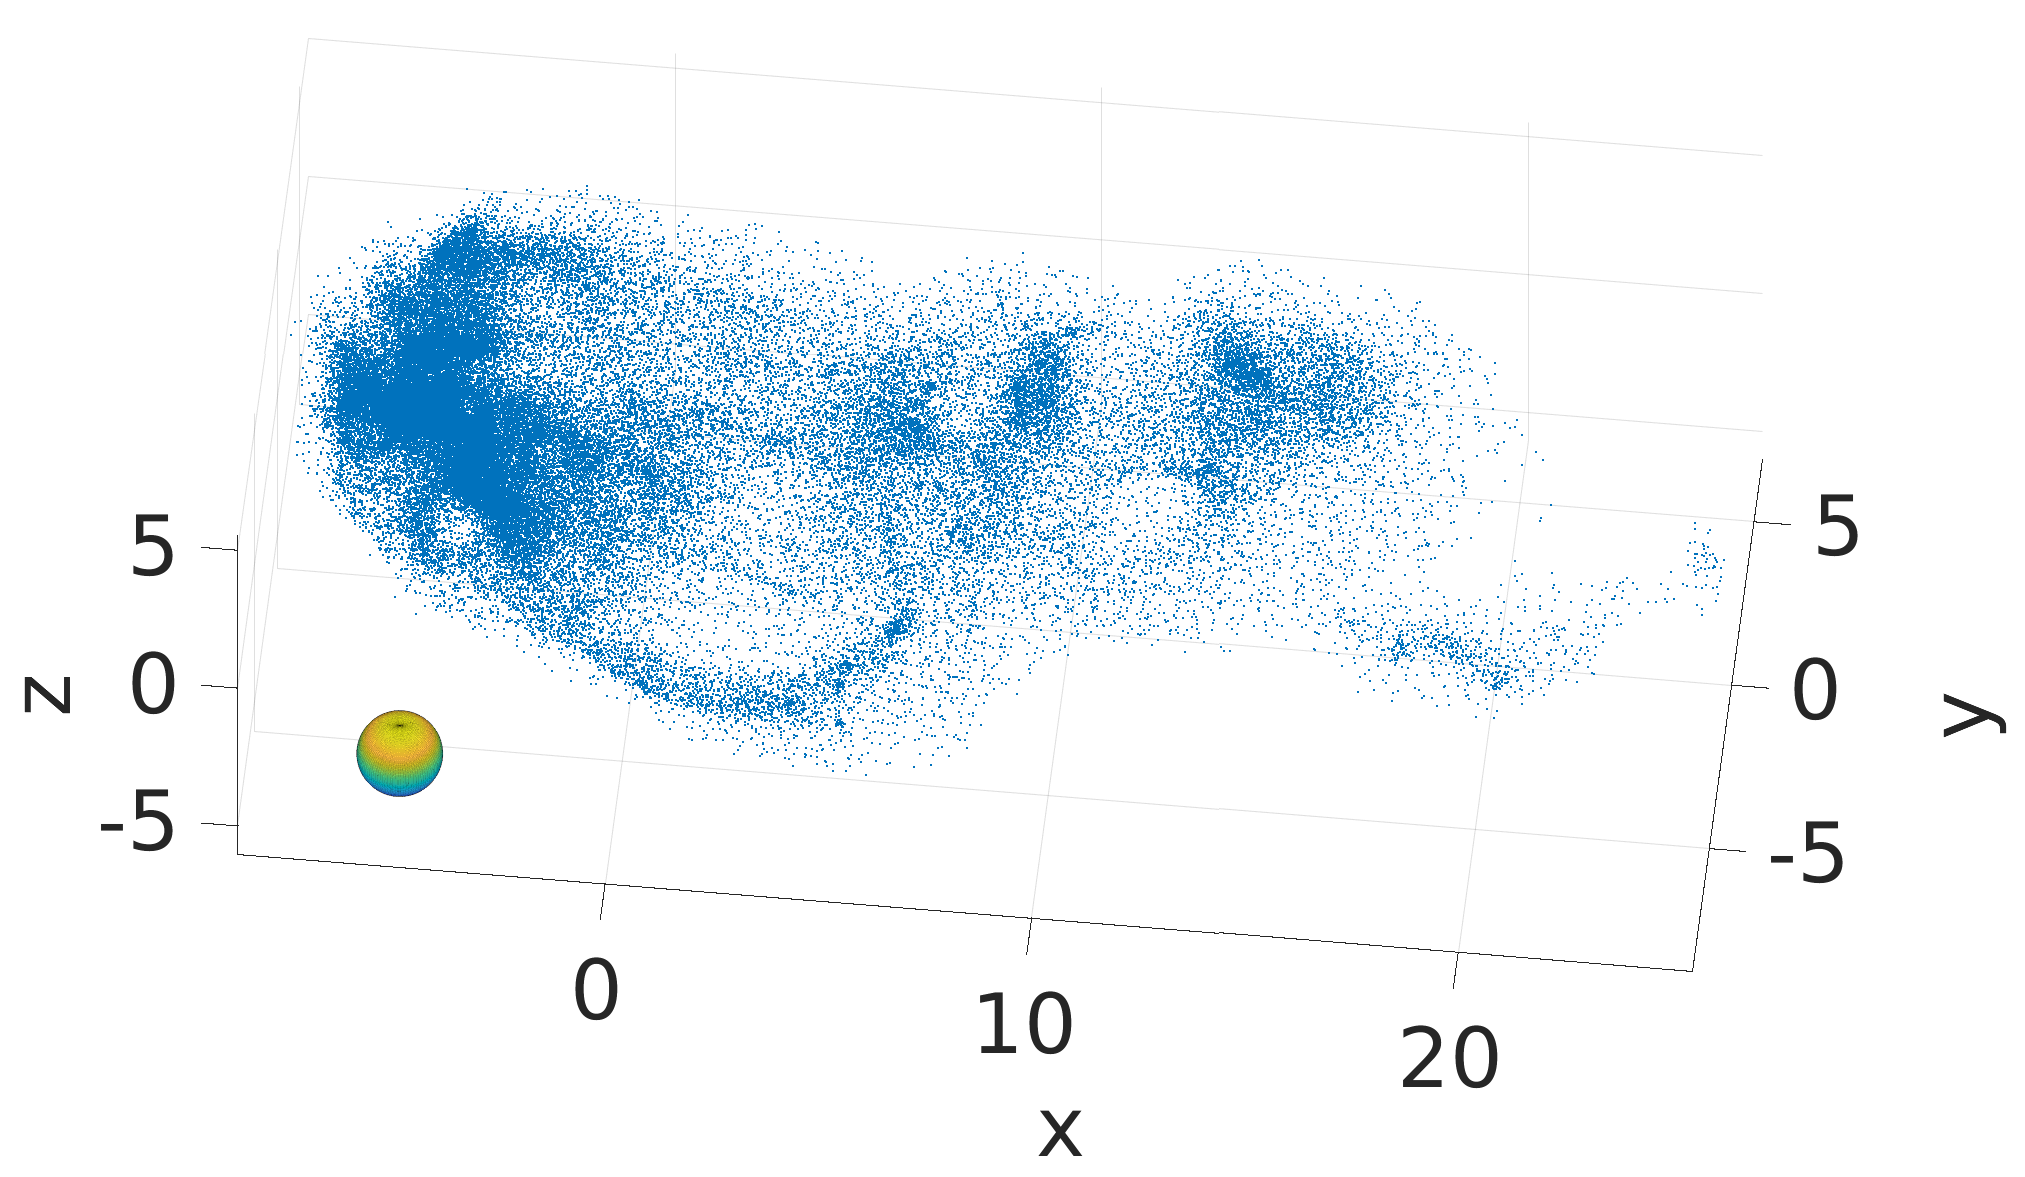
\includegraphics[width=\textwidth]{Figures_png/JF_Dataset}
  \caption{Gas particles of the simulated dwarf galaxy falling into the halo of the Fornax Galaxy Cluster.}
  \label{fig:JF_Dataset}
\end{figure}

Starting from the suite of simulations of dwarf galaxies evolving in a Fornax-like cluster environment (explained in detail in Chapter \ref{ch:simulations}), we chose a single simulated snapshot representing an irregular, gas rich galaxy, exposing an elongated star forming gaseous tail during intense ram pressure stripping (we used a snapshot at $\tau=0.97, t=12.1$~Gyr of simulation ID 69).
% We want to investigate the geometry of their star forming regions.
% The simulation is performed using a modified version of the mixed N-body/Smoothed Particle Hydrodynamics (SPH) code GADGET-2 \cite{Springel_2005, DeRijcke2013}.
% The simulation output consists of three types of particles: Dark Matter (DM), stellar and gaseous.
% In particular, we will concentrate on morphology of gas with density $\rho \ge 10^{-3} ~ \mathrm{atoms/cm^3}$,
%which is a
%since this is a reasonable condition for it to be visible in the observed electromagnetic bandwidth.
\begin{figure}[ht]
    \centering
    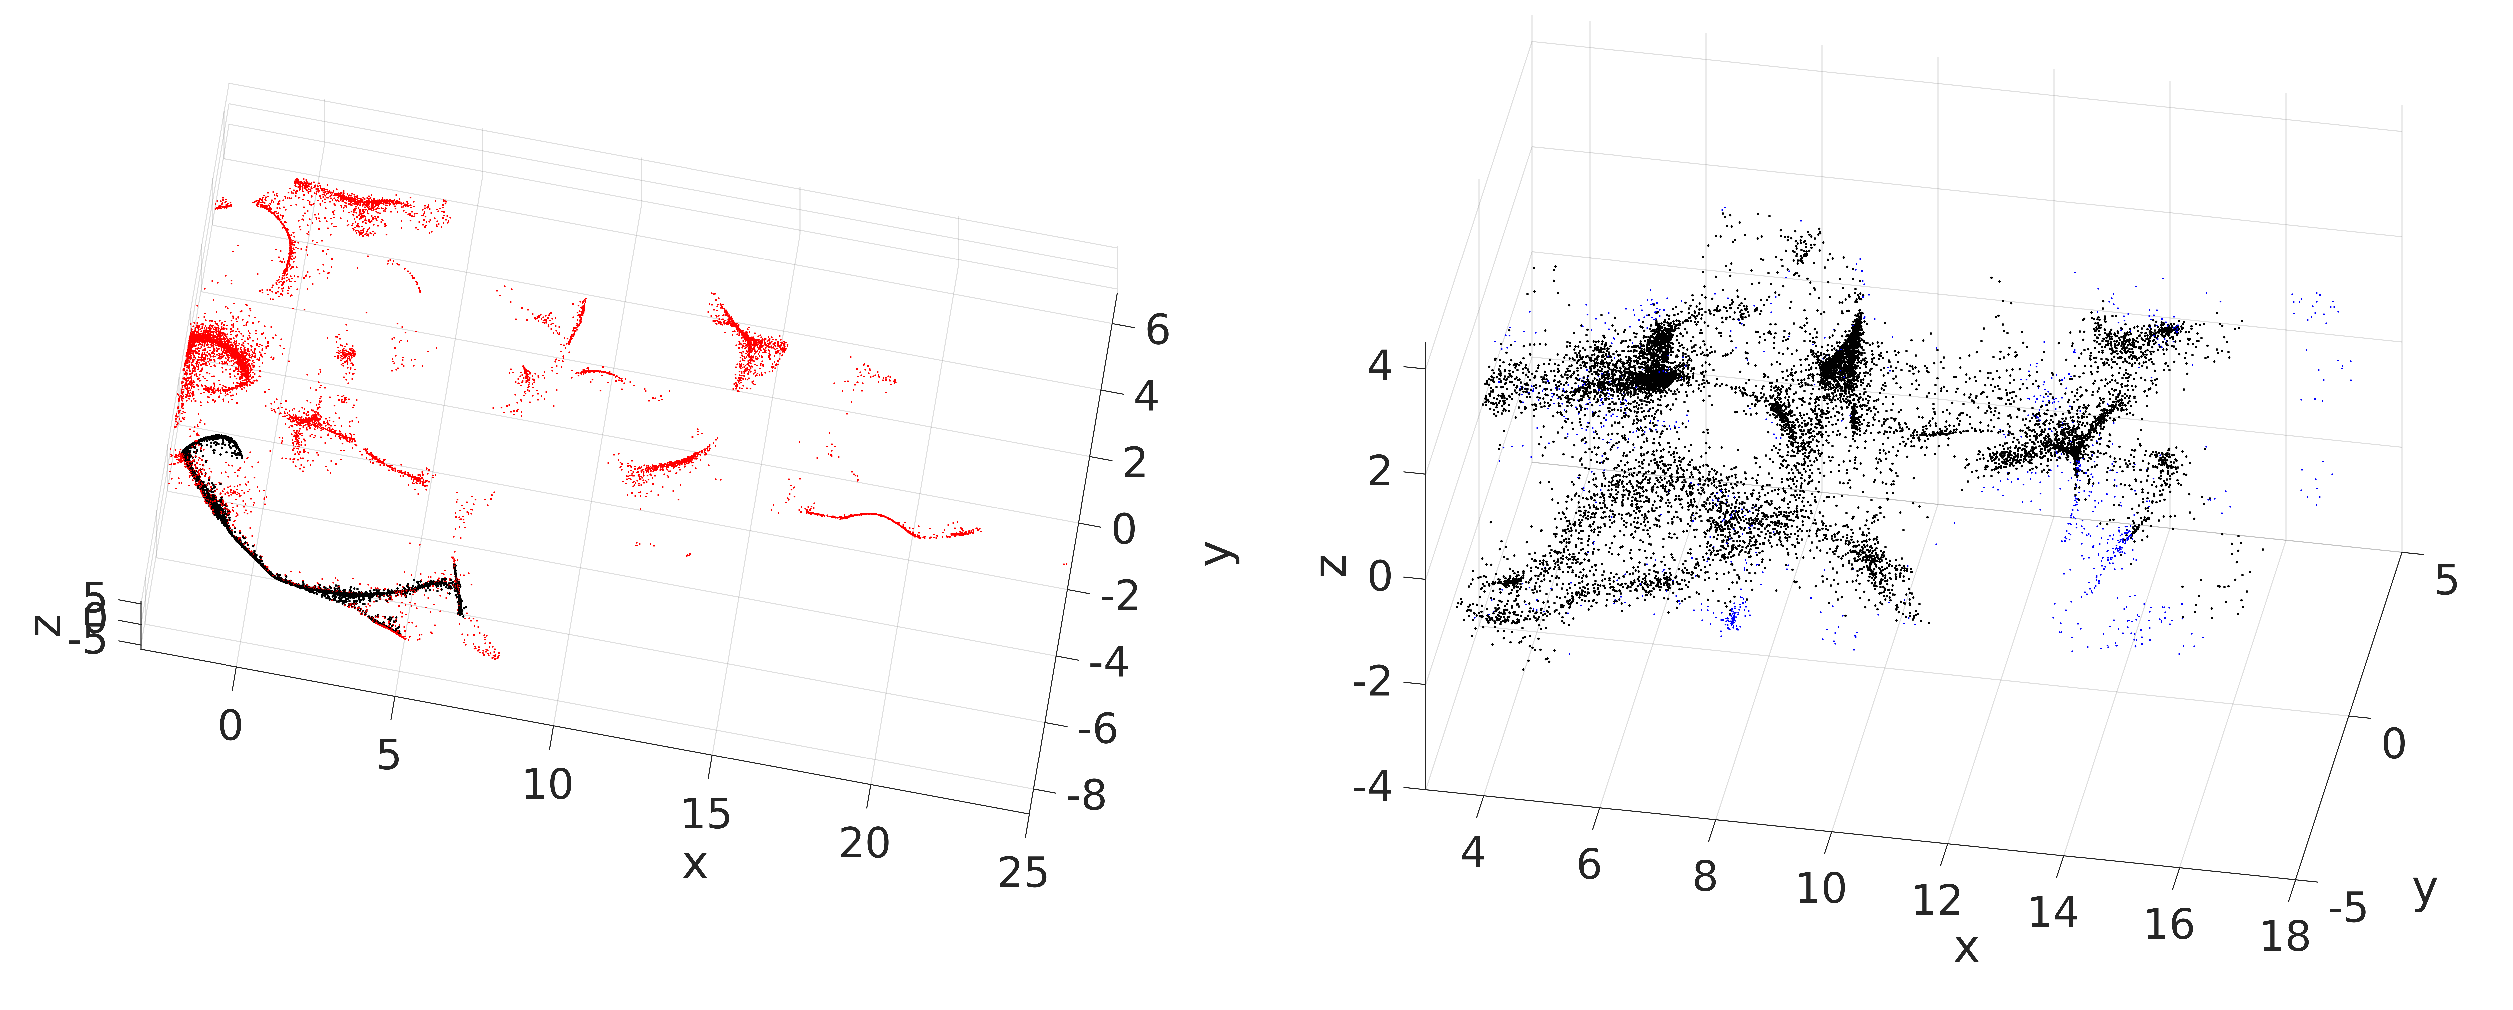
\includegraphics[width=\textwidth]{Figures_png/JF_SAF_Index_Man_v3}
    \caption{1-D (left) and 2-D (right) distributions of the diffused particles in the tail of the jellyfish structure.
    Highlighted in black are the points belonging to two distinct 1-D and 2-D structures discussed in section \ref{sec:manifold_jellyfish}.}
    \label{fig:JF_Res}
\end{figure}
% We disregard DM and stellar particles (needed for evolution of the object, but not relevant for our analysis) and concentrate on the distribution of gas particles.
As described in Section \ref{sec:SPH}, the computation model in SPH simulations is based on a particle formulation of hydrodynamics where each particle samples physical properties of a volume of radius $r_N$ - radius of the sphere containing $N$ neighbouring particles.
A continuous distribution of the physical variables over the full domain is then obtained by spatial smoothing with Gaussian kernels centered on each particle \citep{1977MNRAS.181..375G}.
Associated with each gas particle are values of physical quantities such as density, temperature, pressure etc.

To do this we post process the simulation obtaining for each particle the intensity of the \cii{} emission line.
This is the ``forbidden" line emitted by a carbon atom which has been ionized - having 5 out of 6 electrons.
The outermost electron of the ionized atom gets excited on a higher energy level by radiation.
The excited electron, under extremely low density environment conditions, is able to re-emit radiation at a specific wavelength ($158 ~ \mathrm{\mu m}$) while jumping to a lower energy level.
These types of emission lines are called ``forbidden" due to their impossibility to be seen in normal terrestrial environments.
%They are, however, commonly observed in astronomy ([HII], O[III], etc.).


An estimate of \cii{} emission in  this kind of simulations is obtained by using evolved quantities of the gas (metallicity, density and temperature) as inputs of chemical evolution models of the radiating gas, taking into account its ionization equilibrium and ion level occupation model \citep{Maio2007, DeRijcke2013}.

The resulting gas particle data set is presented in Figure \ref{fig:JF_Dataset}.
Several low dimensional structures are clearly visible, for example the long 1-D manifold departing from the head and elongating along the $x$-axis of the simulation box.
Visually inspecting the data set, we chose a radius $r~=~1~\mathrm{kpc}$ as the characteristic scale parameter for the manifolds (shown as the small sphere in Figure \ref{fig:JF_Dataset}).
The chosen radius is in agreement with the spatial resolution of recent observations.
The parameter $r$ is fixed for preprocessing through diffusion and filtering (section \ref{sec:SAF}), local dimensionality estimation (section \ref{sec:D_Index}) and manifold crawling (section \ref{sec:Crawling}).
% The other parameters are set as in the synthetic data experiments of section \ref{subsec:MulitCrawl}: $\epsilon=1$, $\eta=0.75$ and $\beta=0.4$.

As mentioned earlier, the main body of the data set can be visually divided into head and tail parts.
However, from the topological standpoint there is no justification for clear segregation into 1-D manifolds in the tail and 2-D manifolds in the head.
Dimensionality index estimation clearly identified 1-D structures in the tail, such as the elongated stream of particles starting from the head.
However, points in the head were also predominantly identified as 1-D, due to its complicated, intertwined filamentary structure.
On the other hand, distribution of 2-D points was more localized in the main body of the tail.


\section{A multi-manifold analysis of a dwarf jellyfish galaxy}\label{sec:manifold_jellyfish}

Having obtained the multi-manifold probabilistic profile of the gas particles in the tail of the jellyfish galaxy,
it is possible to perform various kinds of detailed analysis of how physical properties vary along the manifolds.
Here we concentrate on the curvature (Figure \ref{fig:curvatureJF}), computed through the embedding (details in \citet{Canducci2021} and on the star formation potential.
The latter is analysed by studying the the behaviour of emission line \cii{} over the 1-D and 2-D structures
in the jellyfish tail shown as black dots in Figure~\ref{fig:JF_Res} (left) and (right), respectively
- the gaseous stream of gas particles departing from the head and reaching half way through the tail and the predominant 2-D structure in the tail.
\begin{figure}[ht]
  \centering
  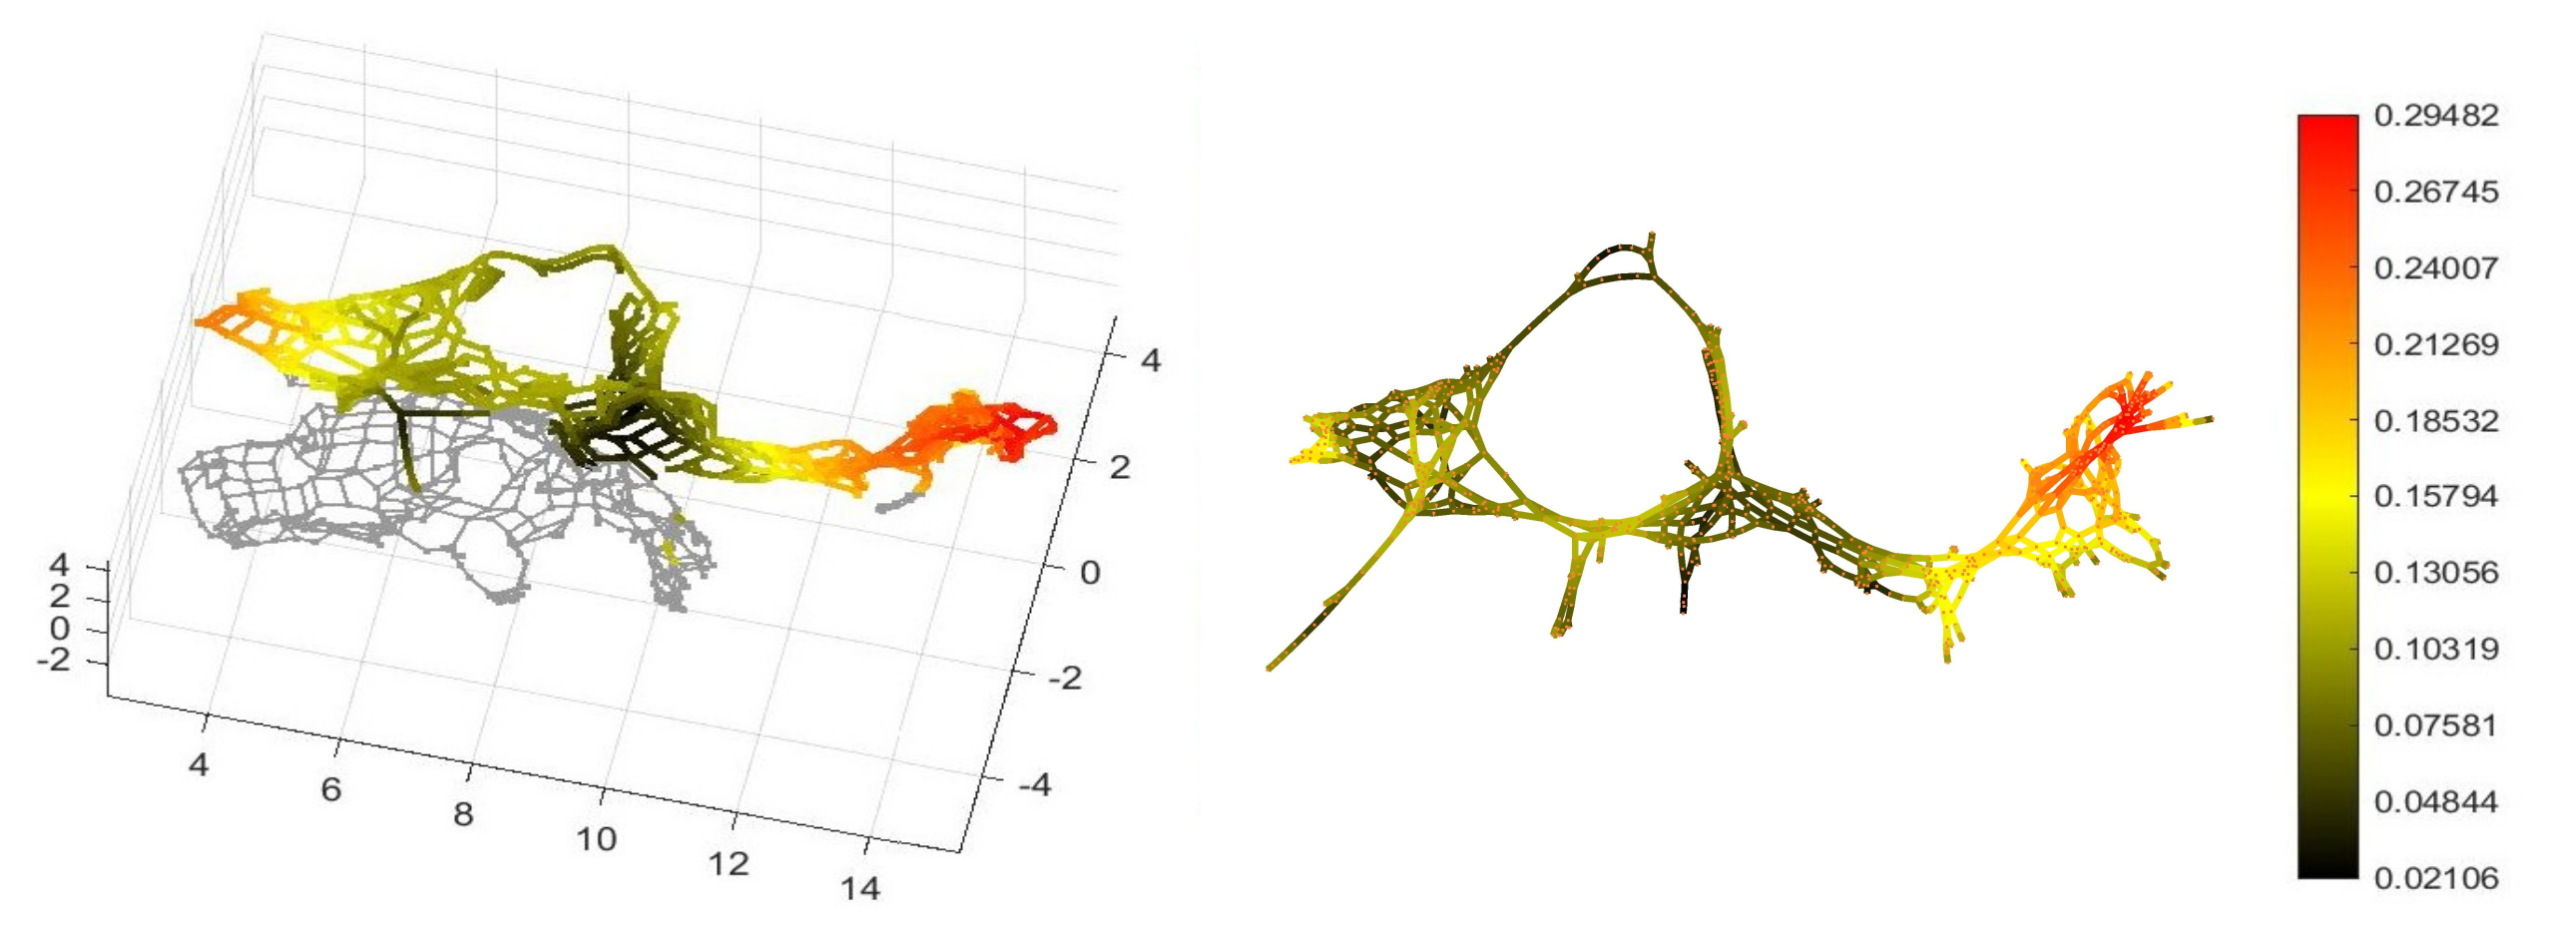
\includegraphics[width=\textwidth]{Figures_png/JF_TotalCurvature_Man2d.png}
  \caption{Embedded graph (left panel) and planar representation (right panel) of a 2-dimensional manifold extracted from the jellyfish data set.
  The local curvature for each vertex is shown in color.}
\label{fig:curvatureJF}
\end{figure}

Figure \ref{fig:curvatureJF}, left panel shows two regions of high curvature, for the 2-dimensional manifold presented in Figure \ref{fig:JF_Res}, right panel.
The far right region of intense curvature, is located towards the end of the tail, where the gas motion is more chaotic due to the motion of the galaxy through the halo of the galaxy cluster. However, the spherical region on the left side of the manifold, presenting a coherent curvature throughout its elongation (top right corner of Figure \ref{fig:curvatureJF}) suggests, as a possible cause of formation, an isotropic expansion, typical of Supernova remnants.

We performed the SAF filtering dimensionality analysis and manifold crawling, and for an identified manifold we show in Figure \ref{subfig:1dManGraph} the embedded vertices
$\bar{\vect{v}}_j$ of the graph $\bar{\cal G}$
for the stream model.
The color codes are the intensity modulated by the weighted mean of \cii{} values $\mathcal{I}^{\text{\cii{}}}_i$ of particles $\vect{t}_i$ in the manifold, using the SPH smoothing kernel $W$ defined in equation \eqref{eq:cubicspline} in Section \ref{sec:density_estimation}:
%\begin{equation}\label{eq:WeightedVar}
%    \overline{\mathcal{I}}^{\text{\cii{}}}_j = \frac{\sum_{i=1}^{N_{\mathcal{M}}} p(v_j | \vect{t}_i,\zeta_j\Sigma_j,\vect{W}_j) ~ \mathcal{I}^{\mathrm{[CII]}}_i}{\sum_{k=1}^{N_{\mathcal{M}}} p(v_j | \vect{t}_k,\zeta_j\Sigma_j,\vect{W}_j)}
%\end{equation}
\begin{equation}\label{eq:WeightedVar}
  \overline{\mathcal{I}}^{\text{\cii{}}}_j = \frac{\sum_{i=1}^{N} \mathcal{I}^{\text{\cii{}}}_i W (\norm{\vect{t}_i - \bar{\vect{v}}_j}, h_i) m_i/\rho_i }{\sum_{k=1}^{N} W ({\vect{t}_i - \bar{\vect{v}}_j}, h_i) m_i/ \rho_i}
\end{equation}
Analogous diagram for the 2-D structure is presented in Figure \ref{subfig:2dManGraph}.

In the 1-D case, the manifold is located at the outskirts of the Jellyfish (Figure~\ref{fig:JF_Dataset}, left panel),
meaning that it is more exposed during the evolution to the surrounding gas of the galaxy cluster.
This implies that the manifold is subject to a higher ram pressure than the tail, leading to a higher density and lower temperature of the gas - necessary conditions for the formation of new stars.
These conditions are reflected in an increase of the \cii{} emission line over the middle section of the manifold, $3 < x < 6$, thus informing us of an enhanced star formation rate, compared to the rest of the manifold.
\begin{figure}[ht]
\centering
\begin{subfigure}[t]{0.48\textwidth}
 \caption{}
 \label{subfig:1dManGraph}
 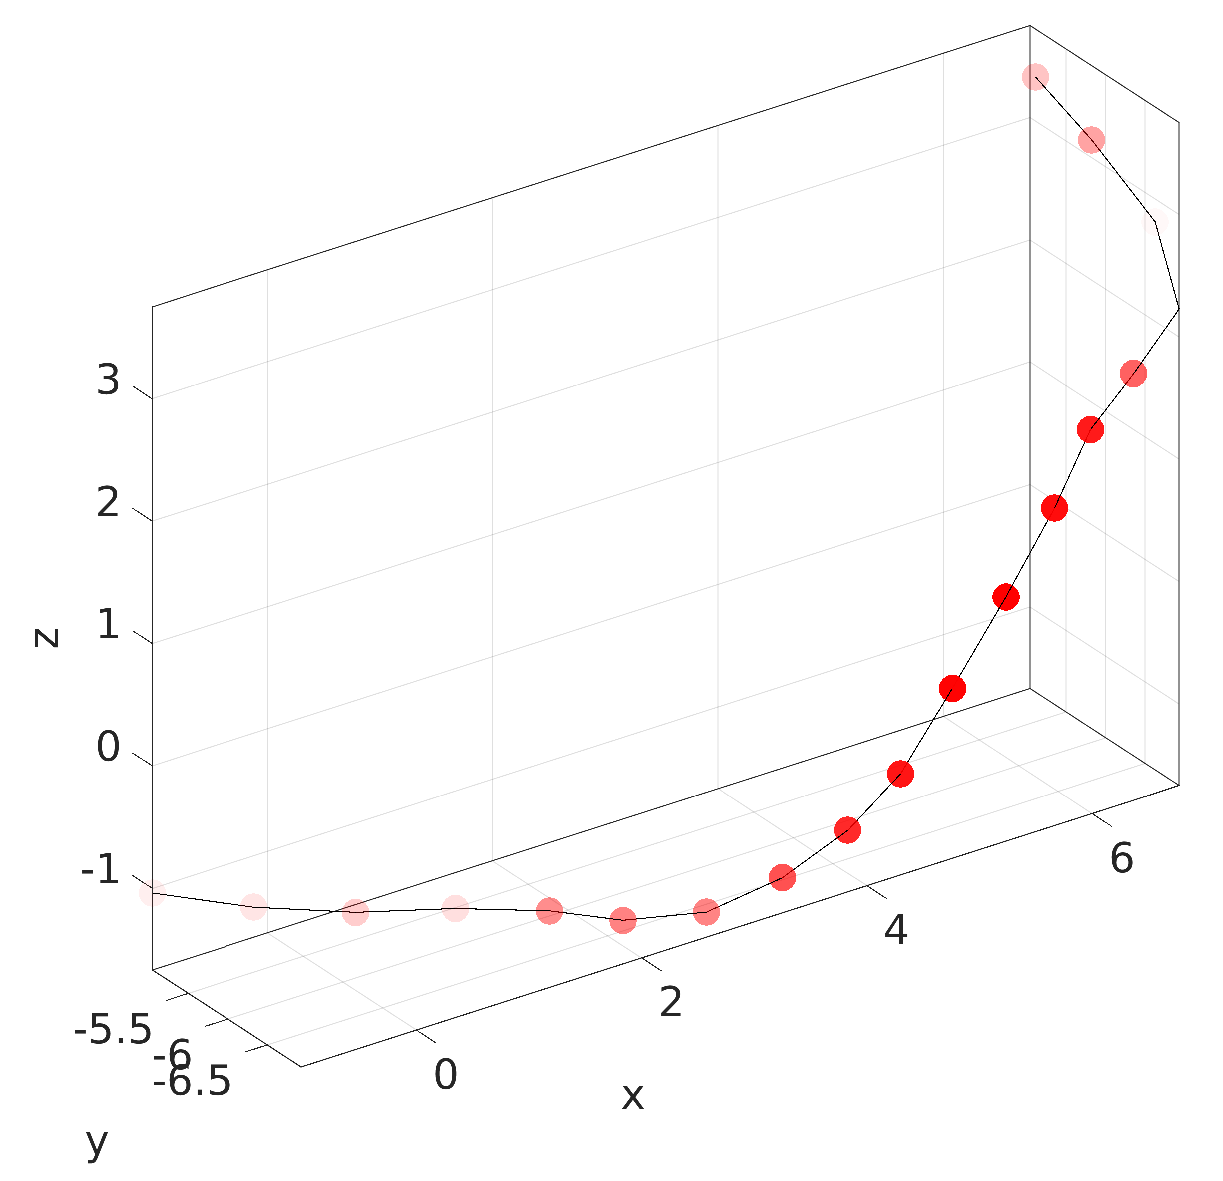
\includegraphics[width=\textwidth]{Figures_png/Manifold1D_AGTM2_cii_Shading}
\end{subfigure}
\begin{subfigure}[t]{0.49\textwidth}
 \caption{}
 \label{subfig:2dManGraph}
 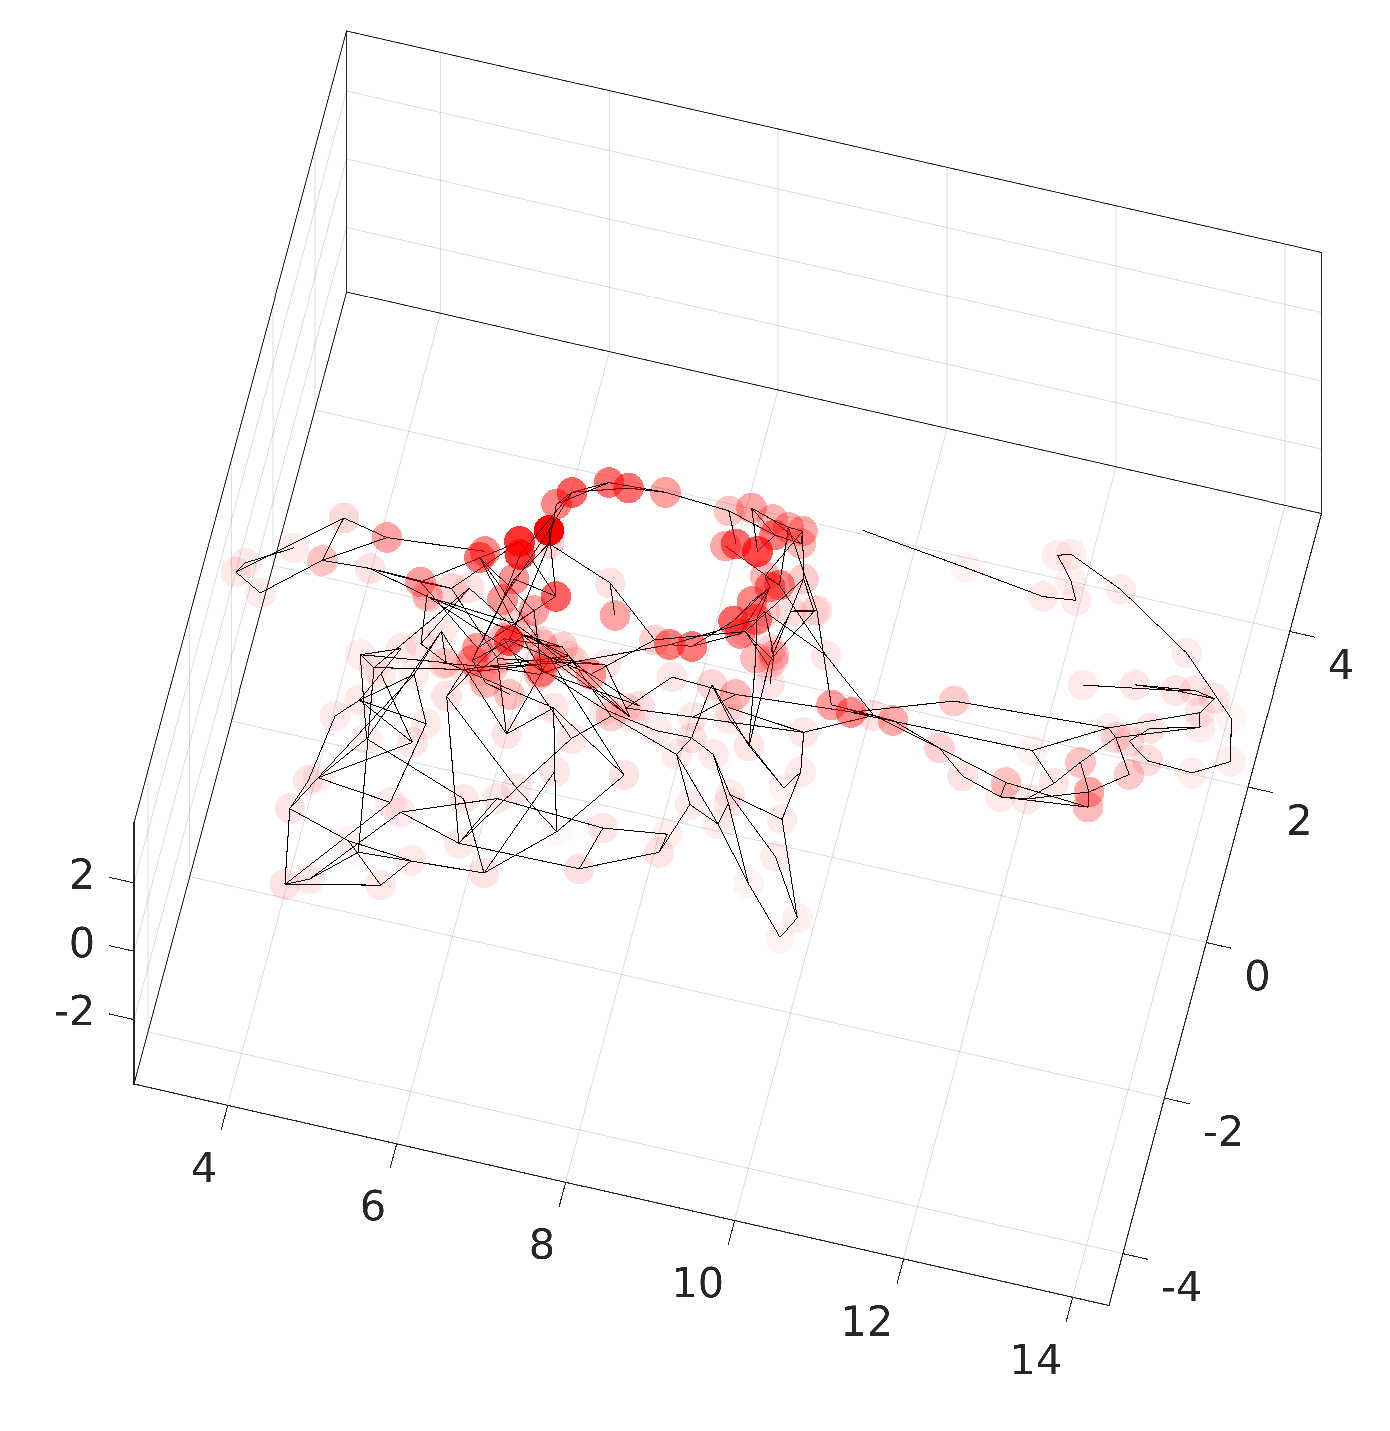
\includegraphics[width=\textwidth]{Figures_png/Manifold2D_AGTM2_cii_Shading}
\end{subfigure}
\caption{1-D (a) and 2-D (b) manifolds extracted from the data set in Figure~\ref{fig:JF_Dataset}.
The graphs' nodes are colored based on the value of \cii{} of the surrounding particles lying not further than $\mathrm{1~kpc}$ from the local tangent space of the manifold, weighted by the nodes' responsibilities.}
\label{fig:Man2D}
\end{figure}
The 2-D structure shows an overall constant \cii{} intensity whereas the region at $5 < x < 9$ presents sharply higher values.
The shape of this region is particularly interesting. It is, in fact, a hole with an almost spherical section.
This structure detected with Manifold Crawling, with potent \cii{} emission at its boundary, is the remnant of a supernova explosion.
Due to their high mass, young stars burn efficiently and relatively fast all their gas reservoir, terminating their life as supernovae and injecting energy and debris in the surroundings.
This process is modeled in the simulation via an injection of $10^{51}$~erg of energy for a short amount of time and a transfer of metallic elements (in the case of our simulation, the model tracks iron and magnesium, \cite{DeRijcke2013}) to the neighbouring gas particles.
The metal-enriched gas particles (like in the surrounding of a supernova explosion) are then able to cool down more efficiently and show strong \cii{} emission line.

Our methodology provides a strong tool for extracting such an information from the morphology of gas particles and can be used to effectively calibrate feedback models in simulations.

Such a detailed analysis of low dimensional structures (remnants of galaxy interactions) is not currently possible with tools routinely used to calibrate and analyse astrophysical simulations of galaxy evolution.
The technique presented in this paper can be used as a semi-automatic exploratory tool by the domain experts, where the focus and characteristic scale of the structures to be mined can be varied continuously with analysis of their physical properties of interest (after necessary computations) performed and studied on the fly.
As an example we show an application in the next section.

\section{Evolution of quantities along the jellyfish tails}

%simulation ID 69 snapshot 180.

%After optimization of the parameters of SGTM through the E-M algorithm, every manifold $\cM_k$ is represented as a gaussian mixture with manifold aligned noise, whose updated centers $\{\ti_{\ell}; \ell = 1,\dots,L^k\}$ are constrained to lie on a 1-dimensional subspace of $\RR^3$.
We now describe a methodology that, taking full advantage of the manifold extraction technique and SPH density formulation, simultaneously recovers the behaviour of simulated properties along the manifold's elongation and its thickness within the simulated volume.
In this section we consider only the 1-D case.
It's possible to carry out a similar analysis for the 2-D case, but
the result is not of easy interpretation and not appropriate in this context.

We start from the centers found by the crawling which are lying on the identified manifold. These center are points $\ti_{\ell} \in \tilde{\mathcal{Q}}$ belonging to the diffused dataset.
From each pair of adjacent centers we can compute the tangent bundle on the 1-D manifold:
\begin{equation}
  \hat{\vect{v}}_{\ell} =  \frac{\ti_{\ell + 1} - \ti_{\ell}}{|| \ti_{\ell + 1} - \ti_{\ell}||},
\end{equation}
The norm $d_{\ell} = || \ti_{\ell + 1} - \ti_{\ell}||$ is also the distance between the two adjacent centers.

\subsection{Computing a point cloud around each manifold segment}
Around each segment of length $d_{\ell}$ we want to build a cylinder or randomly distributed points which will be used to compute tangential and radial average along the manifold of the quantity.
To do so, let us now consider a point cloud $\cC$ containing randomly distributed points $\vect{p} \in \cC$, uniformly sampling a cylindrical volume of radius $1$, aligned along the $z-$axis and centered at the origin $\cO$.
As a first step we partition the point cloud into concentric cylindrical shells $\cS^i: \bigcup_i \cS^i \equiv \cC$.
For every point $\vect{p} \in \cC$ we compute its distance to the cylinder $z-$axis, versor $\hat k$.
We can now group points in $\cC$ so that:
\begin{equation}
  \cS^i =
  \left\{ \vect{p}_j:  r_{i-1} \leq \norm{\vect{p}_j-\hat{k}} < r_i \right\},\, \forall \vect{p}_j \in \cC.
\end{equation}

\begin{figure}
  \centering
  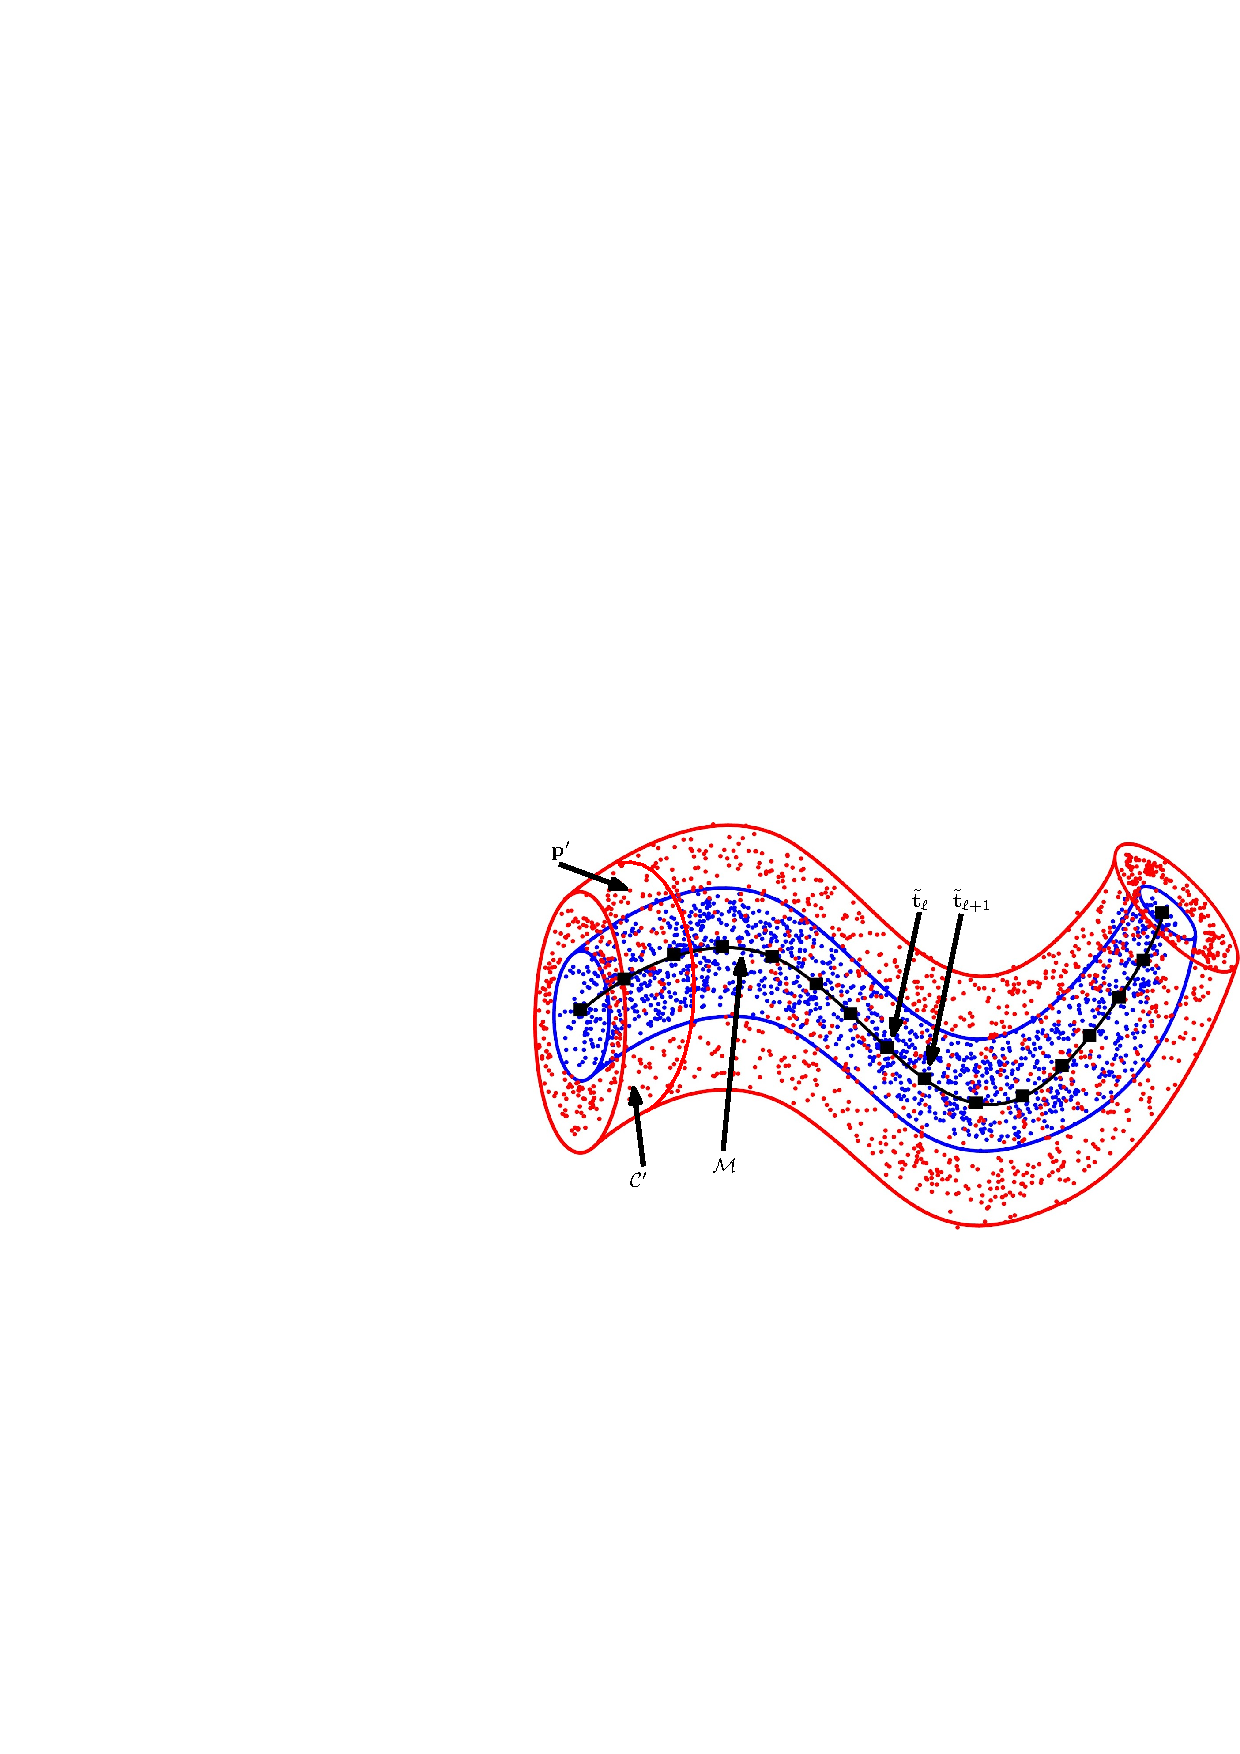
\includegraphics[width=0.8\textwidth]{CylinderAnnotated.pdf}
  \caption{Schematic of the partition of the space around the manifold in two concentric cylindrical shells ($\cS'^1, \cS'^2$) of uniformly distributed sample points $\vect{p}'_i$ constituted by segmented cylinders (only one is shown on the left) build from one center to another of the manifold $\cM$ (in black).}
  \label{fig:cylinder}
\end{figure}

\begin{figure}
  \centering
  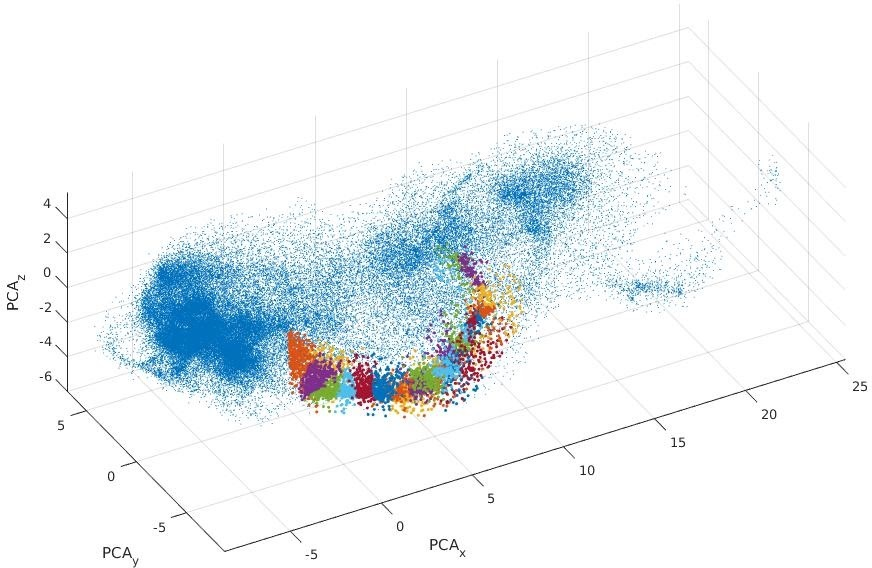
\includegraphics[width=\textwidth]{manifold_partitioned.jpg}
  \caption{Points $\vect{t}_j$ around the identified manifold, coloured differently depending on the longitudinal partition they belong to.}
  \label{fig:segmented_manifold}
\end{figure}

We radially partition into concentric cylindrical shells and for each point we compute its distance to the projected origin, as show in Figure~\ref{fig:cylinder}.

It is always possible to scale, translate and rotate the point cloud so that the cylindrical axis is oriented as the vector $\vect{v}_{\ell}$, the origin over-posed to center $\ti_{\ell}$ and the axis length equal to $d_{\ell}$.
%\paragraph{Scaling}
The scaling operator is the diagonal matrix $S = \diag(1, 1, d_{\ell})$.
%\[
%S =
%\begin{pmatrix}
%  1 & 0 & 0\\
%  0 & 1 & 0\\
%  0 & 0 & d_{\ell}
%\end{pmatrix}
%\]
%\paragraph{Rotation}
To rotate the cylinder we compute the quaternion $\quat{q}$ which rotates the $z-$axis versor $\hat{\vect{k}}$ into $\hat{\vect{v}}_{\ell}$. From equation \eqref{eq:quaternion_from_two_versors}
\begin{equation}
  \quat{q} = \frac{\quat{q^*}}{\norm{\quat{q^*}}} \quad \text{with }
  \quat{q^*} = (\hat{\vect{v}}_{\ell} \vdot \hat{\vect{k}} + 1, \hat{\vect{v}}_{\ell} \cross \hat{\vect{k}}).
\end{equation}
%Its matrix representation is given by R:
%\[
%R =
%\begin{pmatrix}
%  1 - 2q_2^2 - 2q_3^2  &    2q_1q_2 - 2q_3q_4  &   2q_1q_3 + 2q_2q_4\\
%  2q_1q_2 + 2q_3q_4   &    1 - 2q_1^2 - 2q_3^2	&   2q_2q_3 - 2q_1q_4 \\
%  2q_1q_3 - 2q_2q_4	&   2q_2q_3 + 2q_1q_4   &	1 - 2q_1^2 - 2q_2^2
%\end{pmatrix}
%\]
%\paragraph{Shift}
We can then shift the scaled and rotated point cloud so that its origin is on center $\ti_{\ell}$.
Any point $\vect{p} \in \cC$ is then mapped to $\vect{p}' \in \cC'$ under the combined operator as:
\begin{equation}\label{eq:cylOperator}
%  \vect{p}' = (\vect{p} ~ S) ~ R + \ti_\ell
  \vect{p}' = \conj{\quat{q}}(S\,\vect{p})\quat{q} + \ti_\ell
\end{equation}
%}

Having obtained a point cloud $\cC'$ uniformly sampling a thick cylindrical volume with axis tangential to the tangent subspace of manifold $\cM$ on point $\ti_\ell$,
we can now compute the SPH weighted mean of any quantity contained in the data set, over the volume sampled by $\cC'$.
%Note that the families of indices $\cI_1,\dots,\cI_{N^r}$, when applied to $\cC'$, they contain all indices of points in cylindrical shells concentric w.r.t. point $\ti_\ell$ and vector $\vect{v}_{\ell}$, radially partitioning the cylindrical volume sampled by $\cC'$.\\

Consider now a point $\vect{p}' \in \cC'$, we need to compute the weighted mean, under the SPH formalism, of a quantity $V$ summing through all the particles $\vect{t}_j \in \vect{Q}$.
As usual we use the the M-4 spline kernel $W$ defined in equation \eqref{eq:cubicspline} in Section~\ref{sec:density_estimation}.
the exact weighted mean of quantity $V$ at point $\vect{p}'$ is:
\begin{equation}\label{eq:WeightedMean}
  \langle V(\vect{p}') \rangle = \dfrac{\sum\limits_{\vect{t}_j \in \vect{Q}} \dfrac{m_j}{\rho_j} V(\vect{t}_j) W(q_j,h_j)}{\sum\limits_{j=1}^{|\vect{Q}|} \dfrac{m_j}{\rho_j} W(q_j,h_j)}
\end{equation}
where $q_j = \norm{\vect{p}' - \vect{t}_j}/h_j$.
We highlight that the summation is carried out on the whole dataset $\vect{t}_i$.
Given the finite support of the kernel $W$, practically only particles close to the manifold will contribute to $\langle V \rangle$, see Figure~\ref{fig:segmented_manifold}.
The terms in the denominator are generally considered to be approximating unity when the particles in a data set are distributed uniformly; however, this is not often the case in practice.
As mentioned in Section~\ref{sec:SPH}, each particle at position $\vect{t}_j$ of an SPH data set samples a spherical volume of radius $h_j$.
However, all particles are evolved following the equations of motion defined by the Lagrangian formulation of fluids.
Thus, the distribution of particles in a data set at a given evolutionary stage is far from uniform, making the initial assumption incorrect.
The role of the normalization term
%\[\sum_{i =1}^{|\vect{Q}|} \frac{m_j}{\rho_j}W(q_i,h_i)\]
in the denominator of equation \ref{eq:WeightedMean} is to eliminate the dependence of the interpolation to the particle's distribution.
As such, it can not be disregarded when computing the interpolation of quantity $V$ on any point in the volume.
% TODO  Consider to put here the normalization factor now in the SPH section

After computing $\langle V(\vect{p}')\rangle$ for every $\vect{p}' \in \cC'$ we can now evaluate the mean value of $V$ over the concentric cylindrical shells built in the original manifold.% defined by the index families $\cI_1,\dots,\cI_{N^r}$ as:
\begin{equation}
  \langle V(r_{i-1},r_i)\rangle = \frac{1}{|\cS'^i|} \sum_{\vect{p}'_j \in \cS'^i} \langle V(\vect{p}'_j)\rangle,
\end{equation}
obtaining the mean of $V$ over the cylindrical shell between $(r_{i-1},r_i)$.

\begin{sidewaysfigure}
  \centering
  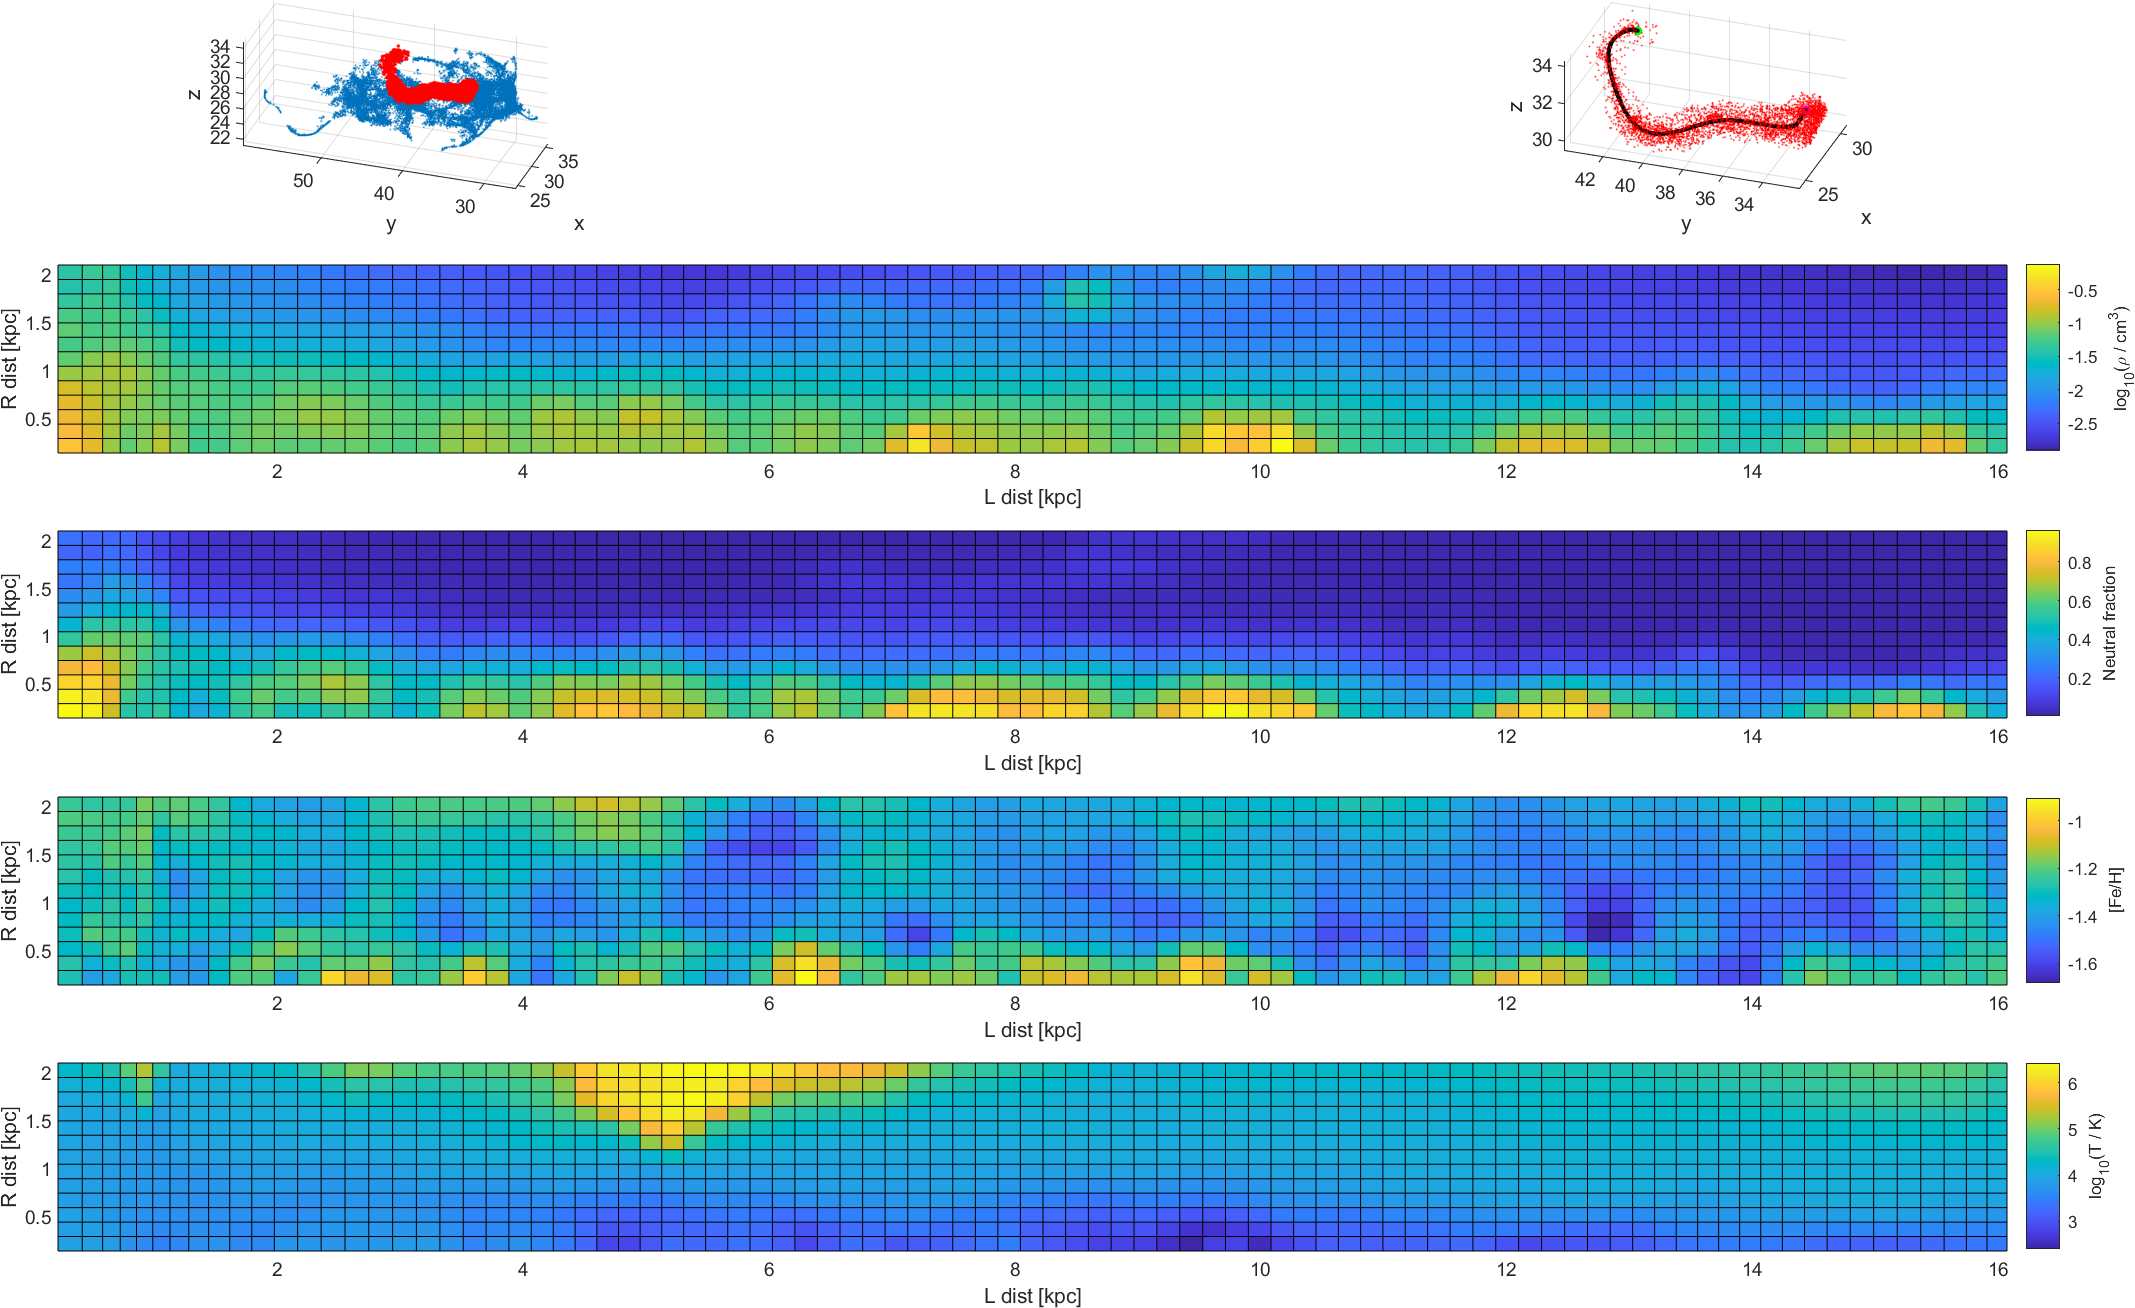
\includegraphics[width=\textwidth]{Figures_png/Manifolds/Manifold4_MeanSubplots_long.png}
  \caption{Longitudinal and radial profiles of different quantities for a long manifold constituting a tentacle of the tail of the jellyfish.
  In the top left corner, the position of the manifold in the diffused dataset is shown in red.
  In the top right corner a detailed view of the non diffused gaseous particle belonging to the manifold.}
  \label{fig:ManifoldLong}
\end{sidewaysfigure}

%\begin{sidewaysfigure}
%  \centering
%  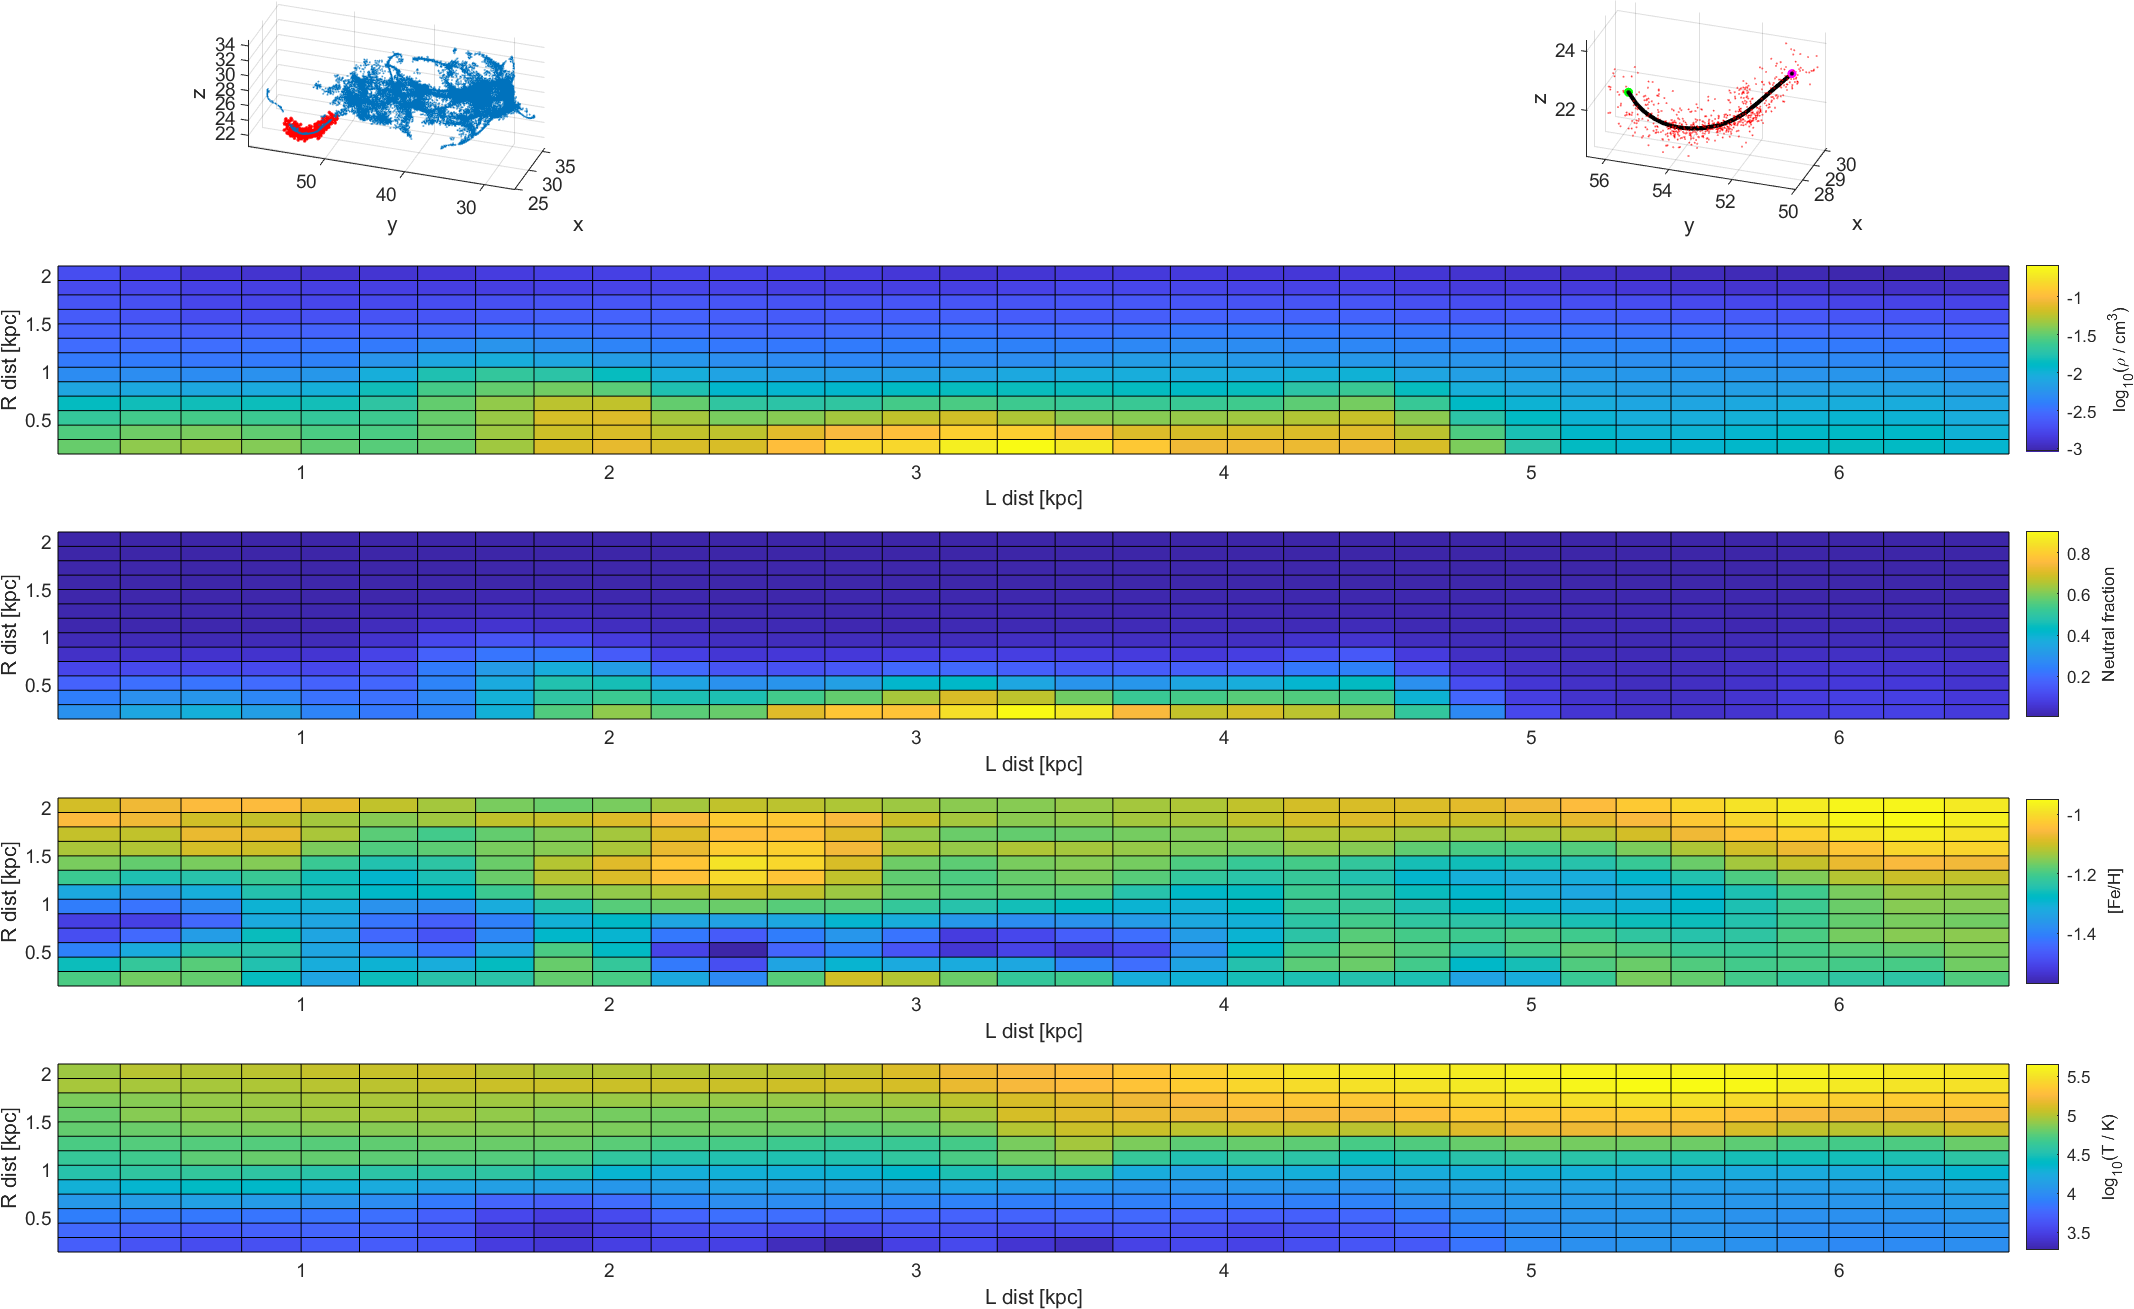
\includegraphics[width=\textwidth]{Figures_png/Manifolds/Manifold1_MeanSubplots.png}
%  \caption{}
%  \label{fig:ManifoldExists}
%\end{sidewaysfigure}

%
% Bi-dimensional profiles for manifolds $\cM_1$ (top row) and $\cM_2$ (bottom row)
%  with and without the normalization term in equation $\ref{eq:WeightedMean}$ (left and right columns respectively), for variables $\overline \rho_i, \overline V_{1i}, \overline V_{2i},$
%  and $\overline m_i$ (top to bottom respectively on each panel).
%  Particularly interesting is the difference in the distribution of the constant scalar value of variable $m$ with and without normalization.

We can iterate the whole process for every center the manifold, obtaining for each linear segment the distribution of $V$ in concentric cylindrical shells.

\subsection{How do quantities vary along the tail manifold?}
By considering both longitudinal profiles (defined along the tangent bundle of the manifold $\cM$, see Figure~\ref{fig:segmented_manifold})
and radial profiles (obtained by the linear operator defined in equation~\eqref{eq:cylOperator} on point cloud $\cC$), we obtain the plots shown in Figure~\ref{fig:ManifoldLong}.% and \ref{fig:ManifoldExists}.
They represents a 1-D manifold detected with the crawling.
In each panel, the vertical axis of the plot contains the radius of the cylindrical shells $r$
and the horizontal axis the approximated geodesic distance (computed by summation of the lengths of the individual linear segments) from the head of the manifold.
The longitudinal axis in the figure goes from the jellyfish head (corresponding to $0$~kpc) to the tail.

In Figure~\ref{fig:ManifoldLong} we show the evolution of volumetric density $\rho$, neutral fraction, iron abundance \feh{} and temperature $T$.
We notice how the central part of the manifold in the radial direction is denser as expected.
The density is high enough to self-shield from the UV background keeping the gas neutral as shown in the second panel.
This suggests that the tail would be visible when viewed in the $21$~cm radio frequency.
Longitudinally, towards the head (left-most part of the plot), density and neutral fraction are larger with respect to the end of the tail.
This is natural given the amount of gas concentrated in the jellyfish head.
The iron abundance distribution is instead characterized with locations of high metallicity, roughly corresponding to high density regions.
They corresponds to regions of recent star formation where supernova feedback has taken place.
This is in line with the hypothesis of galactic tails beaded with knots of star formation in the tail.
Moreover, there is no strong gradient of \feh{} along the tail, suggesting a poor mixing of gas between the galactic tail and the cluster gas.
This is confirmed by the almost uniform distribution of temperature in the tail, where the only high temperature region is a possible infiltration of cluster gas in the tail.

%The bottom plot in each panel presents the mass distribution over the radial and longitudinal dimensions of the manifolds.
%As expected, the mass is constant throughout the sampled volumes and it is everywhere $\overline m_i = 1$.\\
%In order to check the influence of the normalization term we show in Figures \ref{fig:M1_MeanPlots} and \ref{fig:M2_MeanPlots} the corresponding behaviours of $\overline{\rho}_i, \overline{\vect{V}}_{1,i}, \overline{\vect{V}}_{2,i}$ and $\overline m_i$ when the normalization term is omitted in equation \eqref{eq:WeightedMean}.
%While the ranges of the first three variables exceed their true respective values, it is striking the difference of the mass distribution with respect to the normalized versions (Figures \ref{fig:M1_MeanPlotsNorm} and \ref{fig:M2_MeanPlotsNorm}).
